%%% Hlavní soubor. Zde se definují základní parametry a odkazuje se na ostatní části. %%%

%% Verze pro jednostranný tisk:
% Okraje: levý 40mm, pravý 25mm, horní a dolní 25mm
% (ale pozor, LaTeX si sám přidává 1in)
\documentclass[12pt,a4paper]{report}
\setlength\textwidth{145mm}
\setlength\textheight{247mm}
\setlength\oddsidemargin{15mm}
\setlength\evensidemargin{15mm}
\setlength\topmargin{0mm}
\setlength\headsep{0mm}
\setlength\headheight{0mm}
% \openright zařídí, aby následující text začínal na pravé straně knihy
\let\openright=\clearpage

%% Pokud tiskneme oboustranně:
% \documentclass[12pt,a4paper,twoside,openright]{report}
% \setlength\textwidth{145mm}
% \setlength\textheight{247mm}
% \setlength\oddsidemargin{14.2mm}
% \setlength\evensidemargin{0mm}
% \setlength\topmargin{0mm}
% \setlength\headsep{0mm}
% \setlength\headheight{0mm}
% \let\openright=\cleardoublepage

%% Vytváříme PDF/A-2u
\usepackage[a-2u]{pdfx}

%% Přepneme na českou sazbu a fonty Latin Modern
\usepackage[czech]{babel}
\usepackage{lmodern}
\usepackage[T1]{fontenc}
\usepackage{textcomp}

%% Použité kódování znaků: obvykle latin2, cp1250 nebo utf8:
\usepackage[utf8]{inputenc}

%%% Další užitečné balíčky (jsou součástí běžných distribucí LaTeXu)
\usepackage{amsmath}        % rozšíření pro sazbu matematiky
\usepackage{amsfonts}       % matematické fonty
\usepackage{amsthm}         % sazba vět, definic apod.
\usepackage{bbding}         % balíček s nejrůznějšími symboly
			    % (čtverečky, hvězdičky, tužtičky, nůžtičky, ...)
\usepackage{bm}             % tučné symboly (příkaz \bm)
\usepackage{graphicx}       % vkládání obrázků
\usepackage{fancyvrb}       % vylepšené prostředí pro strojové písmo
\usepackage{indentfirst}    % zavede odsazení 1. odstavce kapitoly
\usepackage{natbib}         % zajištuje možnost odkazovat na literaturu
			    % stylem AUTOR (ROK), resp. AUTOR [ČÍSLO]
\usepackage[nottoc]{tocbibind} % zajistí přidání seznamu literatury,
                            % obrázků a tabulek do obsahu
\usepackage{icomma}         % inteligetní čárka v matematickém módu
\usepackage{dcolumn}        % lepší zarovnání sloupců v tabulkách
\usepackage{booktabs}       % lepší vodorovné linky v tabulkách
\usepackage{paralist}       % lepší enumerate a itemize
\usepackage[table,usenames]{xcolor}  % barevná sazba

\usepackage{subcaption}
\usepackage{wrapfig}
%\usepackage{imakeidx}
\usepackage{makeidx}
\makeindex
%\makeindex[program=texindy,options=-L czech -M lang/czech/utf8 -M indexstyle.xdy]

\usepackage{filecontents}
\begin{filecontents*}{instyle.xdy}
;;; xindy style file

;;; Load a predefined style:
;;;(require "makeindex.xdy")


(markup-locclass-list :open ", " :sep "")

(define-attributes (( "textbf" "default" )) )
(markup-locref   :attr  "textbf"     :open "\textbf{\hyperpage{" :close "}}")
(markup-locref   :attr  "textit"     :open "\textit{\hyperpage{" :close "}}")
(markup-locref   :attr  "textttt"     :open "\textttt{\hyperpage{" :close "}}")
(markup-locref   :attr  "texttsc"     :open "\texttsc{\hyperpage{" :close "}}")
(markup-locref   :attr  "default"     :open "\hyperpage{" :close "}")



\end{filecontents*}
\usepackage{longtable}

%%% Údaje o práci

\def\problemy{{\noindent\bf Problémy}\par\bigskip}
\def\TODO#1{{\bf\color{red}#1}\expandafter\expandafter\expandafter\def\expandafter\expandafter\expandafter\problemy\expandafter\expandafter\expandafter{\expandafter\problemy\thepage: #1\par}}
\def\kapitolka#1{
\chapter*{#1}
\addcontentsline{toc}{chapter}{#1}
}
\def\sekcicka#1{
\section*{#1}
\addcontentsline{toc}{section}{#1}
}

% Název práce v jazyce práce (přesně podle zadání)
\def\NazevPrace{Percepční učení a Ideální Bayesovský\jednoumezera pozorovatel při zrakovém vyhledávání}
\def\jednoumezera{\linebreak\par\vglue -14pt\noindent\global\def\jednoumezera{\ }}
% Název práce v angličtině
\def\NazevPraceEN{Perceptual learning and Ideal Bayesian observer in visual search task}

% Jméno autora
\def\AutorPrace{Viktor Němeček}

% Rok odevzdání
\def\RokOdevzdani{2018}

% Název katedry nebo ústavu, kde byla práce oficiálně zadána
% (dle Organizační struktury MFF UK, případně plný název pracoviště mimo MFF)
\def\Katedra{Katedra softwaru a výuky informatiky}
\def\KatedraEN{Department of Software and Computer Science Education}

% Jedná se o katedru (department) nebo o ústav (institute)?
\def\TypPracoviste{Katedra}
\def\TypPracovisteEN{Department}

% Vedoucí práce: Jméno a příjmení s~tituly
\def\Vedouci{Mgr. Filip Děchtěrenko, Ph.D.}

% Pracoviště vedoucího (opět dle Organizační struktury MFF)
\def\KatedraVedouciho{\Katedra}
\def\KatedraVedoucihoEN{\KatedraEN}

% Studijní program a obor
\def\StudijniProgram{Informatika}
\def\StudijniObor{Obecná informatika}

% Nepovinné poděkování (vedoucímu práce, konzultantovi, tomu, kdo
% zapůjčil software, literaturu apod.)
\def\Podekovani{%
Poděkování.
}

% Abstrakt (doporučený rozsah cca 80-200 slov; nejedná se o zadání práce)
\def\Abstrakt{%
Abstrakt.
}
\def\AbstraktEN{%
Abstract.
}

% 3 až 5 klíčových slov (doporučeno), každé uzavřeno ve složených závorkách
\def\KlicovaSlova{%
{klíčová} {slova}
}
\def\KlicovaSlovaEN{%
{key} {words}
}

%% Balíček hyperref, kterým jdou vyrábět klikací odkazy v PDF,
%% ale hlavně ho používáme k uložení metadat do PDF (včetně obsahu).
%% Většinu nastavítek přednastaví balíček pdfx.
\hypersetup{unicode}
\hypersetup{breaklinks=true}

%% Definice různých užitečných maker (viz popis uvnitř souboru)
%%% Tento soubor obsahuje definice různých užitečných maker a prostředí %%%
%%% Další makra připisujte sem, ať nepřekáží v ostatních souborech.     %%%

%%% Drobné úpravy stylu

% Tato makra přesvědčují mírně ošklivým trikem LaTeX, aby hlavičky kapitol
% sázel příčetněji a nevynechával nad nimi spoustu místa. Směle ignorujte.
\makeatletter
\def\@makechapterhead#1{
  {\parindent \z@ \raggedright \normalfont
   \Huge\bfseries \thechapter. #1
   \par\nobreak
   \vskip 20\p@
}}
\def\@makeschapterhead#1{
  {\parindent \z@ \raggedright \normalfont
   \Huge\bfseries #1
   \par\nobreak
   \vskip 20\p@
}}
\makeatother

% Toto makro definuje kapitolu, která není očíslovaná, ale je uvedena v obsahu.
\def\chapwithtoc#1{
\chapter*{#1}
\addcontentsline{toc}{chapter}{#1}
}

% Trochu volnější nastavení dělení slov, než je default.
\lefthyphenmin=2
\righthyphenmin=2

% Zapne černé "slimáky" na koncích řádků, které přetekly, abychom si
% jich lépe všimli.
\overfullrule=1mm

%%% Makra pro definice, věty, tvrzení, příklady, ... (vyžaduje baliček amsthm)

\theoremstyle{plain}
\newtheorem{veta}{Věta}
\newtheorem{lemma}[veta]{Lemma}
\newtheorem{tvrz}[veta]{Tvrzení}

\theoremstyle{plain}
\newtheorem{definice}{Definice}

\theoremstyle{remark}
\newtheorem*{dusl}{Důsledek}
\newtheorem*{pozn}{Poznámka}
\newtheorem*{prikl}{Příklad}

%%% Prostředí pro důkazy

\newenvironment{dukaz}{
  \par\medskip\noindent
  \textit{Důkaz}.
}{
\newline
\rightline{$\square$}  % nebo \SquareCastShadowBottomRight z balíčku bbding
}

%%% Prostředí pro sazbu kódu, případně vstupu/výstupu počítačových
%%% programů. (Vyžaduje balíček fancyvrb -- fancy verbatim.)

\DefineVerbatimEnvironment{code}{Verbatim}{fontsize=\small, frame=single}

%%% Prostor reálných, resp. přirozených čísel
\newcommand{\R}{\mathbb{R}}
\newcommand{\N}{\mathbb{N}}

%%% Užitečné operátory pro statistiku a pravděpodobnost
\DeclareMathOperator{\pr}{\textsf{P}}
\DeclareMathOperator{\E}{\textsf{E}\,}
\DeclareMathOperator{\var}{\textrm{var}}
\DeclareMathOperator{\sd}{\textrm{sd}}

%%% Příkaz pro transpozici vektoru/matice
\newcommand{\T}[1]{#1^\top}

%%% Vychytávky pro matematiku
\newcommand{\goto}{\rightarrow}
\newcommand{\gotop}{\stackrel{P}{\longrightarrow}}
\newcommand{\maon}[1]{o(n^{#1})}
\newcommand{\abs}[1]{\left|{#1}\right|}
\newcommand{\dint}{\int_0^\tau\!\!\int_0^\tau}
\newcommand{\isqr}[1]{\frac{1}{\sqrt{#1}}}

%%% Vychytávky pro tabulky
\newcommand{\pulrad}[1]{\raisebox{1.5ex}[0pt]{#1}}
\newcommand{\mc}[1]{\multicolumn{1}{c}{#1}}


%% Titulní strana a různé povinné informační strany
\begin{document}
%%% Titulní strana práce a další povinné informační strany

%%% Titulní strana práce

\pagestyle{empty}
\hypersetup{pageanchor=false}

\begin{center}

\centerline{\mbox{
\includegraphics[width=166mm]{../img/logo-cs.pdf}}}

\vspace{-8mm}
\vfill

{\bf\Large BAKALÁŘSKÁ PRÁCE}

\vfill

{\LARGE\AutorPrace}

\vspace{15mm}

{\LARGE\bfseries\NazevPrace}

\vfill

\Katedra

\vfill

\begin{tabular}{rl}

Vedoucí bakalářské práce: & \Vedouci \\
\noalign{\vspace{2mm}}
Studijní program: & \StudijniProgram \\
\noalign{\vspace{2mm}}
Studijní obor: & \StudijniObor \\
\end{tabular}

\vfill

% Zde doplňte rok
Praha \RokOdevzdani

\end{center}

\newpage

%%% Následuje vevázaný list -- kopie podepsaného "Zadání bakalářské práce".
%%% Toto zadání NENÍ součástí elektronické verze práce, nescanovat.

%%% Strana s čestným prohlášením k bakalářské práci

\openright
\hypersetup{pageanchor=true}
\pagestyle{plain}
\pagenumbering{roman}
\vglue 0pt plus 1fill

\noindent
Prohlašuji, že jsem tuto bakalářskou práci vypracoval(a) samostatně a výhradně
s~použitím citovaných pramenů, literatury a dalších odborných zdrojů.

\medskip\noindent
Beru na~vědomí, že se na moji práci vztahují práva a povinnosti vyplývající
ze zákona č. 121/2000 Sb., autorského zákona v~platném znění, zejména skutečnost,
že Univerzita Karlova má právo na~uzavření licenční smlouvy o~užití této
práce jako školního díla podle §60 odst. 1 autorského zákona.

\vspace{10mm}

\hbox{\hbox to 0.5\hsize{%
V ........ dne ............
\hss}\hbox to 0.5\hsize{%
Podpis autora
\hss}}

\vspace{20mm}
\newpage

%%% Poděkování

\openright

\noindent
\Podekovani

\newpage

%%% Povinná informační strana bakalářské práce

\openright

\vbox to 0.5\vsize{
\setlength\parindent{0mm}
\setlength\parskip{5mm}

Název práce:
\NazevPrace

Autor:
\AutorPrace

\TypPracoviste:
\Katedra

Vedoucí bakalářské práce:
\Vedouci, \KatedraVedouciho

Abstrakt:
\Abstrakt

Klíčová slova:
\KlicovaSlova

\vss}\nobreak\vbox to 0.49\vsize{
\setlength\parindent{0mm}
\setlength\parskip{5mm}

Title:
\NazevPraceEN

Author:
\AutorPrace

\TypPracovisteEN:
\KatedraEN

Supervisor:
\Vedouci, \KatedraVedoucihoEN

Abstract:
\AbstraktEN

Keywords:
\KlicovaSlovaEN

\vss}

\newpage

\openright
\pagestyle{plain}
\pagenumbering{arabic}
\setcounter{page}{1}


%%% Strana s automaticky generovaným obsahem bakalářské práce

\tableofcontents

%%% Jednotlivé kapitoly práce jsou pro přehlednost uloženy v samostatných souborech
\chapter*{Úvod}
\addcontentsline{toc}{chapter}{Úvod}

Jedna z činností, kterou provádíme mnohokrát denně, je zrakové vyhledáváni.
Proto také existují mnohé výzkumy o tom, jak člověk zrakové vyhledávání
provádí. Jeden z oborů, který se o zrakové vyhledávání zajímá, je psychofyzika.

Jedním z úkolů, který se řeší, je vyhledávání konkrétního cíle v kruhovém poli.
Najemnik a Geisler \citeyearpar{Najemnik05} v nedávné době představili model
Ideálního Bayesovského pozorovatele, který modeluje chování lidského
pozorovatele s překvapivou přesností. Algoritmus, pomocí kterého Ideální
Bayesovský pozorovatel vybíral lokace, které zkoumat, byl ale kubický v počtu
možných lokací cíle. Ve svém pozdějším článku \citep{Najemnik09} 
představili pozorovatele ELM, který Ideálního Bayesovského pozorovatele dobře
aproximuje, a navíc pracuje v kvadratickém čase.

V této práci se podíváme na dva dosud neřešené problémy. Prvním z nich je, zda se lidští
pozorovatelé chovají stejně, když se musí vědomě rozhodovat, jaké na jaké místo
se ve kterém kroku podívají. Druhou, navazující otázkou je, zda se člověk naučí
cíl hledat lépe, když to bude sám zkoušet, nebo když při učení dostane navíc po každém pohledu
informaci o tom, jak dobře si vybral místo, na které se podíval, srovnáním s hodnotou, kterou
tomuto bodu přiřazuje hodnotící funkce ELM pozorovatele.

\section*{Struktura práce}
\addcontentsline{toc}{section}{Struktura práce}

V první kapitole jsou představeny pojmy, teorie a starší výsledky, které tato
práce využívá. V druhé kapitole jsou představeny cíle práce. V následující
kapitole je popsána metodika experimentu. Poté jsou prezentovány vizualizace
naměřených dat, nad nimiž je následně provedena diskuse. K práci jsou též
přiloženy dvě přílohy. V první z nich jsou další grafy z naměřených dat, v
druhé se nachází dokumentace aplikace, prostřednictvím které byl prováděn
experiment a jejíž vznik byl součástí této práce.


\chapter{Teoretický úvod}

V této kapitole přiblížíme některé pojmy a teorie, které jsou v práci využity.

\section{Zrakové vyhledávání}

V úloze zrakového vyhledávání je úkolem najít ve scéně stimul s určitými
vlastnostmi. Tyto scény mohou být jednoduché, jako například několik černých
úseček na bílém pozadí, kdy je úkolem najít úsečku, která má určitý směr. I
takto jednoduché úlohy ale mají mnoho společného se zrakovým vyhledáváním tak,
jak ho provádíme v běžném životě \citep{VisualSearch}. Mohou ale také být velmi
komplikované a těžko popsatelné, jako například hledání muže v pruhovaném
oblečení, jaké známe z populární úlohy \uv{Kde je Valda?}.  

Předchozí výzkum ukázal, že lidští
pozorovatelé v této úloze využívají krátkých pohledů a rychlých pohybů očí \citep{Holmquist}.
Jednomu takovému krátkému pohledu budeme říkat \emph{fixace}. Rychlému očnímu pohybu
se říká \emph{sakáda} \citep{sakady}.

Při vyhledávání nás ve skutečnosti zajímá, ke kterým místům pozorovatel obrací
svou pozornost. To však výrazně souvisí s tím, kam se kouká \citep{Attention}.


\section{Úvod do teorie detekce signálu}

Jeden z dílčích problémů úlohy zrakového vyhledávání je rozlišení hledaného
objektu a pozadí. K popisu řešení tohoto problému se nám bude hodit
terminologie teorie detekce signálu, která se právě touto problematikou
zaobírá.

V řeči této teorie budeme hledanému objektu říkat {\it signál},
rušivým elementům ve scéně se říká {\it šum}. Problém rozlišení hledaného
objektu a pozadí se tedy v řeči teorie detekce signálu formulují jako dotaz,
zda se v dané lokaci signál nachází, či nenachází. Tomuto problému se říká Yes-No
problém \citep{NeilSDT}, nebo pouze Y/N.
\index{Yes-No problém} 
\index{Y/N}

V kontextu Yes-No problému mohou po odpovědi pozorovatele nastat čtyři možné situace \citep{GreenSDT}:

\bigskip\noindent
\begin{center}
\begin{tabular}{ccc}
\hline
\hline
& Signál je přítomen & Signál není přítomen \\
\hline
Pozorovatel odpoví kladně &{\it Hit}&{\it False alarm} \\
Pozorovatel odpoví záporně &{\it Miss}&{\it Correct rejection}\\
\hline
\hline
\end{tabular}
\end{center}
\bigskip
\index{Hit}
\index{Miss}
\index{False alarm}
\index{Correct rejection}

 V této úloze se pozorovatel chová tak,
že si zvolí kritérium (někdy též práh odpovědi), které udává, jaká musí být
pravděpodobnost, že signál je přítomen, aby pozorovatel odpověděl kladně \citep[kapitola 1.7]{GreenSDT}.

\def\P#1{\operatorname{P}\left[#1\right]}
\def\E#1{\mathbb{E}\left[#1\right]}
\def\tP#1{\P{\text{#1}}}

Poté pozorovatel provede pozorování, z nějž získá informaci $o$. Situaci
\uv{Pozorovatel získal informaci $o$} označíme jako $O$. Následně spočítá hodnotu
rozhodovací proměnné, tedy spočítá, jaká je pravděpodobnost, že je signál
přítomen. Tvrzení \uv{Signál je přítomen} označíme jako $S$

Tato pravděpodobnost se z Bayesovy věty spočítá jako 
\begin{equation*}
%\begin{multline*}
\P{S| O} = =\frac{\P{O| S}*\P{S}}{\P{O}} 
%\end{multline*}
\end{equation*}
Potom porovná tuto rozhodovací proměnnou s kritériem a podle výsledku tohoto
porovnání odpoví.

Odsud je zřejmé, že zvyšováním kritéria zvyšujeme pravděpodobnost, že nastane
miss, ale snižujeme pravděpodobnost false alarmu.

V souvislosti s Y/N úlohou je ale ještě nutné zavést následující pojmy:

\begin{definice}\label{hitrate}
Mějme pozorovatele $p$ v úloze Y/N. Potom jeho \emph{hit rate\/} $H_p$ definujeme jako $$\P{\text{hit}|\text{Signál je přítomen}}$$ a jeho \emph{False alarm rate\/} $F_p$ jako $$\P{\text{False alarm}|\text{Signál není přítomen}}.$$
\end{definice}
\index{Hit rate}
\index{False alarm rate}

\subsection{Senzitivita}

\index{Senzitivita}
Jedním s dílčích problémů je též určení, jakou rozlišovací schopnost má daný
pozorovatel na daný signál. Zde ale narazíme na problém -- není triviální
najít parametr, který by rozlišovací schopnost pozorovatele dobře popisoval.

Intuitivně bychom chtěli, aby pozorovatel, který má vysokou senzitivitu,
odpovídal ve většině případů správně. Není ale jasné, co to znamená. V předchozí
podkapitole jsme ukázali, že pozorovatel často může zvýšit pravděpodobnost
hitu za cenu zvýšení pravděpodobnosti false alarmu či naopak. My bychom od senzitivity
však chtěli, aby nezávisela na nastavení kritéria.

Proto představíme příklad z praxe, na němž budeme poté ilustrovat výhody a 
nevýhody různých definic senzitivity.

Nechť je pozorovatelem člověk, který není
příliš pozorný a chystá se přejít silnici. Jeho (podvědomým) pozorováním je
informace, která dorazí do jeho mozku z periferií jeho sítnic, a signálem, jehož
přítomnost zkoumá, je, zda přijíždí auto. V takovém případě se v mozku spustí
algoritmus, který převede pozorování na číslo $X$. Poznamenejme, že v mozku je
hodnota tohoto čísla dobře kvantifikovaná, i když je mimo záběr této práce
popisovat, co přesně z fyzikálního hlediska tato hodnota znamená. Pro
porozumění stačí představa, že se jedná o frekvenci určitého druhu impulsu,
které si mezi sebou neurony posílají. Mozek ví, jakou distribuci má náhodná
veličina $X$ v případě, že se auto blíží, a jakou má v případě, že nikoliv.
Podle konkrétní hodnoty $X$ kterou naměřil, se rozhodne, jestli auto přítomno
není, a je tedy bezpečné silnici přejít, nebo zda je pravděpodobnost
přijíždějícího auta dost vysoká na to, aby mělo smysl zvednout hlavu a podívat
se příslušným směrem znovu s cílem získat lepší pozorování.

První intuitivní nápad by byl definovat senzitivitu $s$ jako $$s=\text{Hit rate}.$$
Z předchozího textu by ale mělo být vidět, že
taková definice citlivosti není vhodná -- například pozorovatel, který vždy odpoví
\uv{ano} by měl v tomto případě optimální citlivost. V našem případě bychom tedy za každé situace usoudili, že auto přijíždí a silnici bychom nikdy nepřešli, což jistě nechceme.

Na druhý pokus zkusíme senzitivitu nadefinovat jako poměr hitů a false alarmů,
tedy jako $$s=\frac{\text{Hit rate}}{\text{False alarm rate}}.$$
Optimalizace s ohledem k takovému parametru by ale též vedla k scestnému nastavení
kritéria.\footnote{V typickém případě, který je popsán v následujících
odstavcích, se pro kritérium jdoucí k nekonečnu tento poměr též blíží k
nekonečnu. Dobrý pozorovatel by tedy téměř vždy odpovídal \uv{ne}, optimální
pozorovatel by neexistoval. Kdybychom takové kritérium použili v našem případě, vždy bychom usoudili, že je bezpečné silnici přejít.}

Další možností by bylo charakterizovat pozorovatele jeho poměrem správných
a špatných odpovědí. Zapíšeme-li takový parametr ale vzorcem, zjistíme, že by vypadal jako
$$s=\text{Hit rate}*\P{S} + (1-\text{False alarm rate})*\P{\overline{S}}.$$ 
Taková definice senzitivity též není vhodná, protože potom by citlivost pozorovatele
nezávisela jen na jeho vlastnostech, ale i na pravděpodobnosti, že bude signál přítomen.

Praxe ukazuje, že v těchto situacích je rozdělení veličiny $X$ často dobře
aproximováno normálním rozdělením, a to jak v případě, že signál přítomen je,
tak v případě, že přítomen není. Obě tato normální rozdělení navíc mají v tomto
typickém případě stejný rozptyl a liší se jen svou střední hodnotou \citep{SwetsSDT}. Potom je
přirozenou otázkou ptát se, jaký je rozdíl mezi jejich středními hodnotami (či lépe
rozdíl mezi jejich středními hodnotami vydělený směrodatnou odchylkou).

Právě tuto hodnotu označíme jako hodnotu $d'$. Protože ale ne vždy je rozdělení
normální, musíme nadefinovat hodnotu $d'$ způsobem, která nebude závislá na rozdělení
veličiny $X$.

\begin{definice}\label{dprime}
Nechť má pozorovatel $p$ hit rate $H_p$ a false alarm rate $F_p$ obě ostře mezi jedničkou a nulou. Potom budeme jeho \emph{senzitivitu}
značit $d'$ a spočítáme ji jako $$d' = \Phi^{-1}(H_p) - \Phi^{-1}(F_p),$$ kde $\Phi^{-1}$ je inverzní distribuční funkce normovaného normálního rozdělení.
\end{definice}
\index{d'@$d'$}



\begin{figure}[h!]
  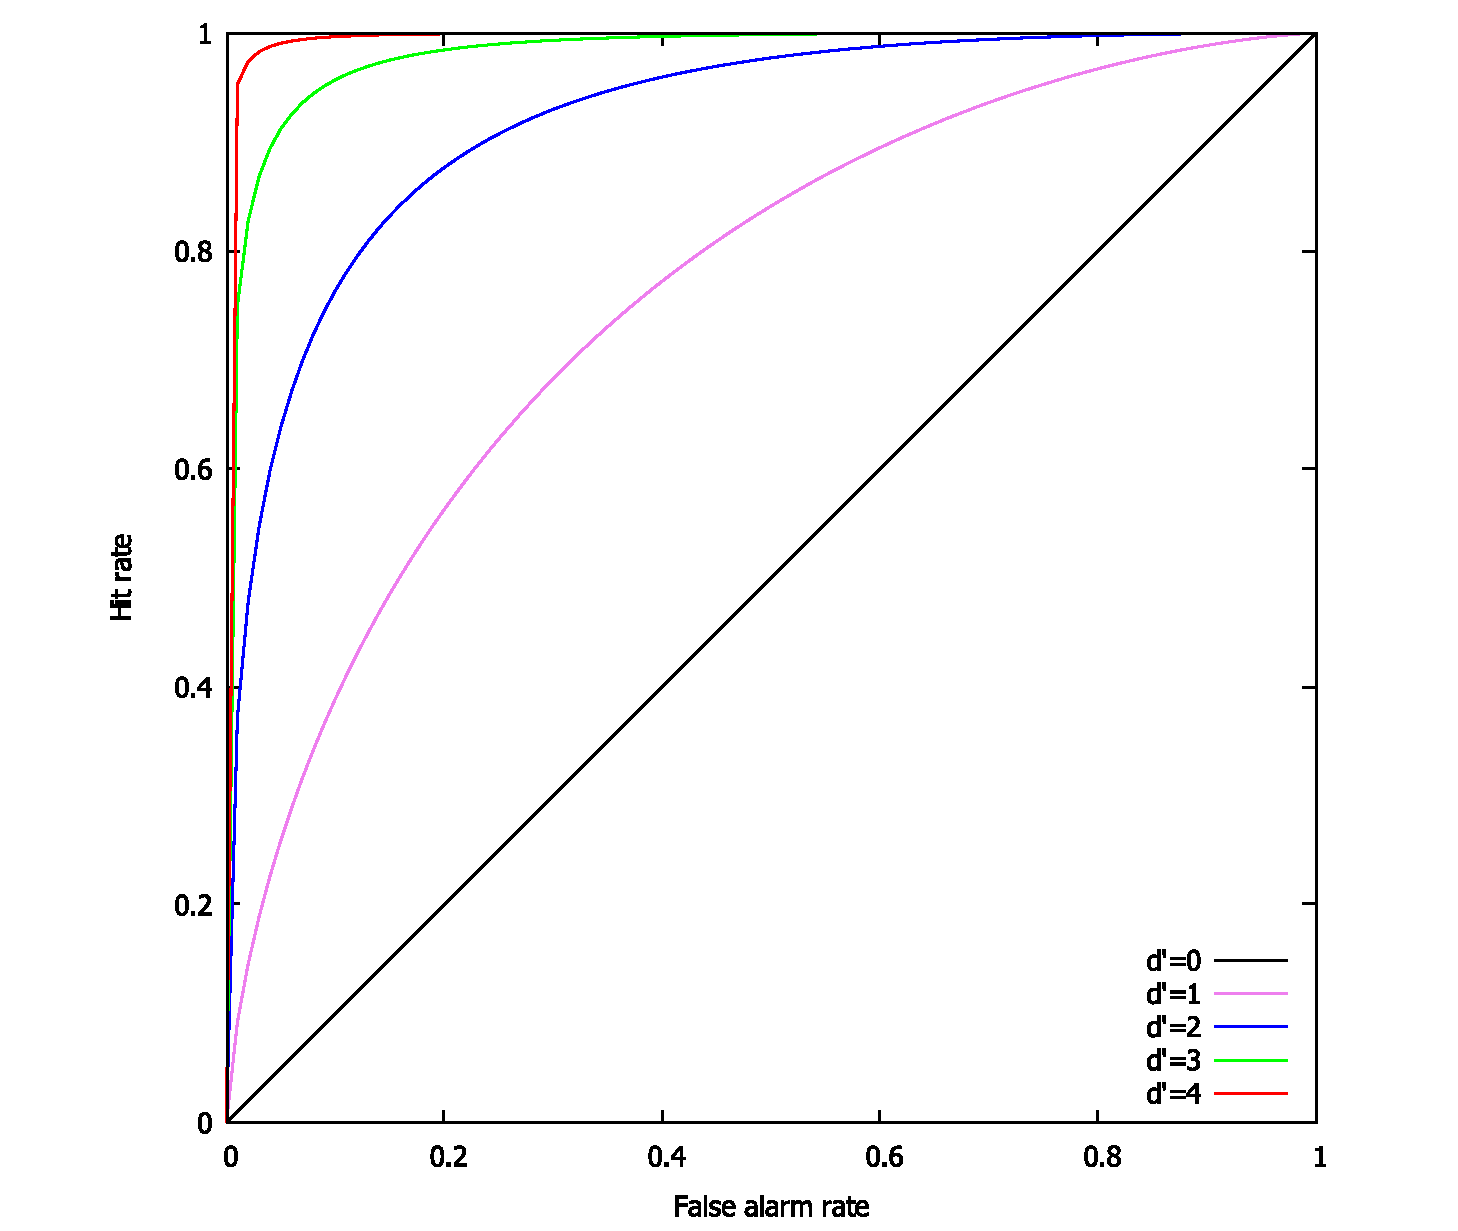
\includegraphics[width=.8\linewidth]{graphs/ROC.pdf}
  \centering
\caption{Závislost hit rate a false alarm rate pro různé hodnoty $d'$. Těmto křivkám se říká ROC křivky z anglického Receiver Operating Characteristic \citep{SwetsSDT,GreenSDT}.} 
\label{obr:dprime} 
\end{figure}


Nahlédneme, že senzitivita má následující vlastnosti:
\begin{itemize}
\item Pokud $d' = 0$, jsou indikátorové náhodné veličiny \uv{Pozorovatel odpověděl kladně} a \uv{Signál je přítomen} nezávislé.
\item Pokud $d' > 0$, mají tyto dvě veličiny kladnou korelaci.
\item Pokud skutečně má náhodná veličina $X$ jak v případě, že signál přítomen je, tak v případě, že signál přítomen není, normální rozdělení lišící se pouze střední hodnotou, pak hodnota $d'$ nezáleží na nastavení kritéria (samozřejmě krom případů, kdy kritérium nastavíme na plus nebo mínus nekonečno, pak hodnota $d'$ není dobře definovaná).
\end{itemize}

Závislost hit rate a false alarm rate pro konkretního pozorovatele se nazývá {\it ROC křivka} z anglického Receiver Operating Characteristic \citep{SwetsSDT,GreenSDT}. ROC křivky pro vybrané hodnoty $d'$ jsou zobrazeny na obrázku \ref{obr:dprime}.  

\section{Šum}

\index{Šum}
V teorii detekce signálu šumem nazýváme nechtěnou (a typicky neznámou)
modifikaci signálu.  Signály a s nimi spojené modifikace můžou být různé
podstaty, například zvukové, nebo se může jednat o šum v elektromagnetickém
vlnění. Také se může na signálu projevit mnoha různými způsoby. Může se k němu
například přičíst. Takový šum nazveme {\it aditivní}. Dále existuje například
 šum multiplikativní či fázový (šum, který se projevuje krátkodobým
fázovým posunem signálu).

Pro úlohu zrakového vyhledávání je relevantní aditivní vizuální šum. Nabízela
by se otázka, proč nepoužít reálnou scénu, nebo naopak jednobarevné pozadí.
Praktické scény jsou však těžko popsatelné a jednobarevné scény (obsahující
pouze diskrétní rozptýlení) vnášejí do formalizace vyhledávání nepřesnosti --
jejich popis je však nad rámec této práce, lze ho najít v článku
\citep{WhyNoise}.

  

\subsection{Barva šumu}

I když však
odhlédneme od média, v němž se šum šíří či v něm je zachycený, existuje mnoho
různých šumů. Jeden z parametrů, který lze měřit, se nazývá {\it výkonová
spektrální hustota}. Její jednotkou jsou watty na Hertz a udává, jaký výkon má šum na dané frekvenci. Máme-li hodnoty šumu v dostatečně mnoha bodech, jeho spektrální hustotu spočítáme tak, že na šum aplikujeme
Fourierovu transformaci.

V závislosti na distribuci výkonu napříč různými frekvencemi přiřadíme šumu jméno. Tato jména jsou (i pro jiný než vizuální šum) odvozena od analogie s viditelným světlem -- šum se pojmenuje podle barvy, jakou by mělo světlo se stejným rozdělením výkonu napříč viditelným spektrem, jaké má šum rozdělení výkonu napříč svým spektrem. Takto známe například bílý, růžový, červený (někdy též označovaný jako
Brownův či nesprávně hnědý\footnote{V anglické literatuře se používá
termín {\it Brownian noise}, setkáme se ale i se zavádějícím
termínem {\it Brown noise}. Jméno je odvozeno od souvislostí s Brownovým pohybem částic}) či modrý šum (viz obrázek \ref{obr:noise:example}).
\index{Šum!bílý}
\index{Šum!červený}
\index{Šum!růžový}
\index{Šum!modrý}

Spektrální hustota $p$ všech zmíněných šumů na dané frekvenci $f$ lze vyjádřit jako
$p=1/f^\beta$, kde hodnota $\beta$ je $-1$ pro modrý šum, $0$ pro bílý, $1$ pro
růžový a $2$ pro hnědý. Proto se růžový šum někdy též označuje jako $1/f$ šum. Pro
ostatní barvy šumu není podobné označení běžné. O šumu a jeho barvách je pojednáno více v
knize Noise \citep{Noise}.

Pravděpodobnostní rozdělení jednotlivých složek Fourierovy transformace ale
není definicí barvy šumu dáno. Pokud je rozdělení normální (Fourierova obrazu nebo samotného šumu), řekneme, že se jedná o Gaussovský šum.

V této práci se budeme zabývat vizuálním šumem, tedy šumem, kde místo obvykle
používané časové souřadnice použijeme dvě souřadnice prostorové a měřenou
hodnotou bude jas. 

\begin{figure}[h!]
\begin{tabular}{cc}
\begin{subfigure}{0.45\textwidth}
  \centering
  
\includegraphics[width=.8\linewidth]{img/blue_noise}
  \caption{Modrý šum} 
\end{subfigure}&
\begin{subfigure}{0.45\textwidth}
  \centering
  
\includegraphics[width=.8\linewidth]{img/white_noise}
  \caption{Bílý šum} 
\end{subfigure}\\
\begin{subfigure}{0.45\textwidth}
  \centering
  
\includegraphics[width=.8\linewidth]{img/pink_noise}
  \caption{Růžový šum} 
\end{subfigure}&
\begin{subfigure}{0.45\textwidth}
  \centering
  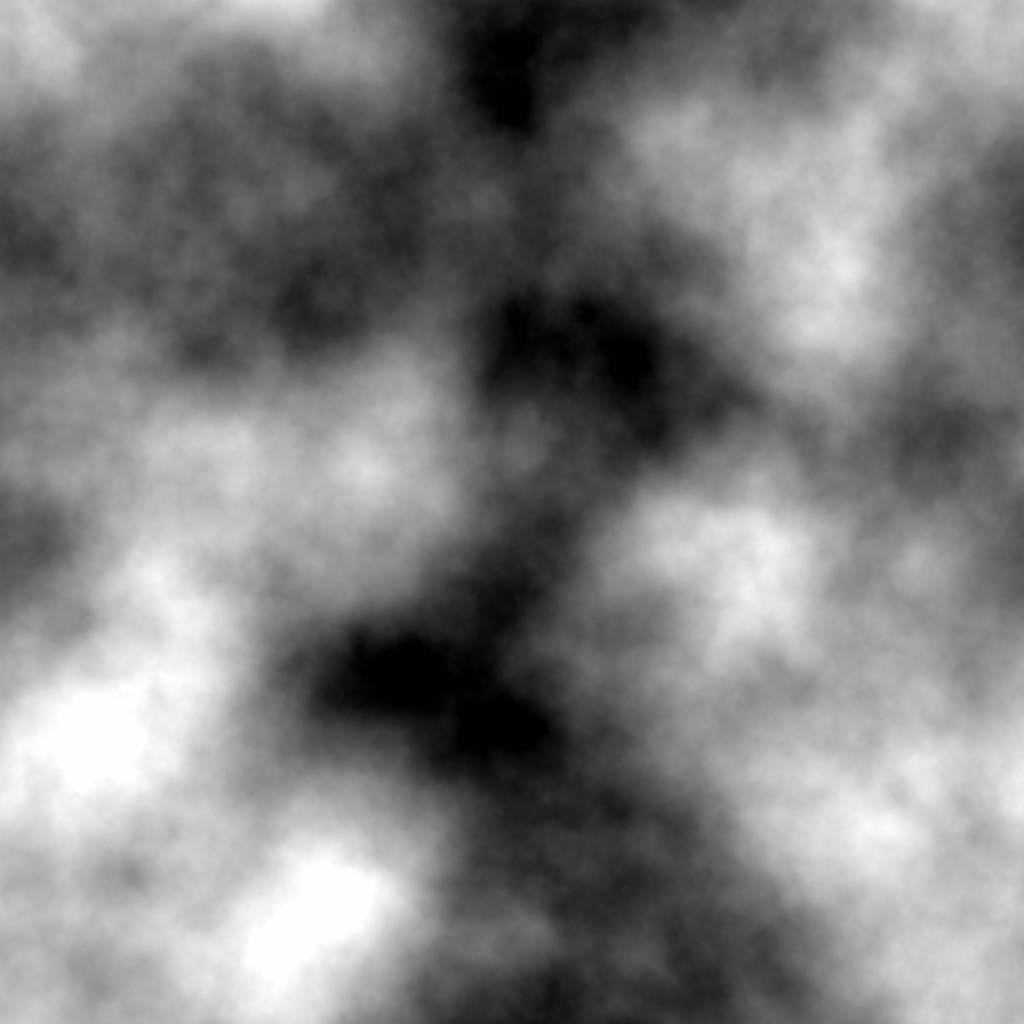
\includegraphics[width=.8\linewidth]{img/brown_noise}
  \caption{Červený, někdy též Brownův šum} 
\end{subfigure}%
\end{tabular} 
\caption{Ukázky různých šumů. Tyto šumy byly vygenerovány pomocí algoritmu použitého přímo v aplikaci, která je součástí této práce. Algoritmus je blíže popsán ve druhé příloze.} 
\label{obr:noise:example} 
 
\end{figure}
\section{Gabor patch}

\index{Gabor patch}

V úloze zrakového vyhledávání potřebujeme také nějaký cíl. V reálném životě
vnímáme mnoho různých podnětů. Pro takovou situaci by však bylo příliš obtížné
najít model. Proto se často používají jednodušší, lépe popsatelné cíle.  Jedním z takových
stimulů je {\it Gabor patch} vycházející z Gabor filteru.

Gabor filter (v českých textech někdy označovaný jako Gaborova vlnka) je
lineární filtr používaný ve zpracování obrazu, chceme-li detekovat signál
mající danou frekvenci a směr, který se vyskytuje kolem daného bodu.

\subsection{Definice}

Hodnotu filtru v daném bodě spočítáme jako součin dvou funkcí. První z nich
nazveme {\it jádro} filtru. Jako jádro se vždy používá sinus či cosinus (někdy
uváděné v podobě komplexní exponenciály, pokud potřebujeme i reálnou, i
imaginární složku). Jeho parametry určují, jaké vlastnosti má mít signál, který
chceme detekovat. Druhé funkci říkáme {\it obálka}, a určuje, na jakém okolí daného
bodu signál zkoumáme.

Funkci tedy lze vyjádřit jako $$g(x,y) =
\sin\left(2\pi\frac{x'}{\lambda}+\phi\right)*\operatorname{obálka}(x',y'),$$
kde vektor $(x',y')$ je vektor $(x,y)$ otočený o úhel, který svírá osa $x$
se směrem, podél nějž chceme měřit signál (tento úhel budeme značit $\Theta$),
a posunutý do bodu, v němž chceme měřit signál, $\lambda$ je frekvence signálu,
který hledáme, a $\phi$ je fázový posun \citep{GaborPatch}. Frekvence signálu
se nejčastěji udává v cyklech na jednotku vzdálenosti, často na pixel obrazu.

Jako obálka se používá dvojrozměrná Gaussova funkce, raised cosine, nebo prostá
lineární funkce vzdálenosti. 

Gaussovu funkci vyjádříme jako $$ \operatorname{obálka}(x,y) =
\exp\left(\frac{x'^2 + y'^2}{2\rho}\right),$$ kde $\rho$ je směrodatná odchylka
Gaussovy křivky. Její výhodou je, že chování Gabor filtru, jehož obálku tvoří
Gaussova funkce, je nejpřesněji popsané. Raised cosine vyjádříme jako 
$$
\operatorname{obálka}(x,y)=
\begin{cases}
 \frac{\cos(\pi\sqrt{x'^2+y'^2}/r)+1}2 &\text{pro $\sqrt{x'^2+y'^2}\leq r$,}\\[1ex]
 0 &\text{jinak,}
\end{cases}
$$ kde $r$ je poloměr oblasti, v níž chceme signál detekovat. Výhodou raised
cosine oproti Gaussově funkci je, že ve vzdálenosti alespoň $r$ od středu
filtru jeho hodnota nabývá nuly. Při výpočtech tedy stačí počítat s malou
oblastí kolem středu (kdežto při použití Gaussovy funkce je nutné počítat s
celým obrazem). Výhodou oproti lineární funkci vzdálenosti je, že raised cosine
se pro většinu aplikací chová dostatečně podobně jako Gaussova funkce.

\subsection{Použití}

Chceme-li detekovat signál ve vizuálním šumu, spočítáme hodnotu $$s=\sum
g(x,y)*n[x,y],$$ kde $n$ je šum a sumu bereme přes všechny body $(x,y)$, v
nichž jsme naměřili hodnoty šumu. Je-li hodnota $s$  blízko nuly, signál v
daném místě není přítomen, nebo je přítomen s jinými parametry. Vysoké hodnoty
značí, že
signál pravděpodobně přítomen je, hluboce záporné značí, že signál je přítomen,
ovšem s fází posunutou $\pi$.

Gabor filter ale můžeme používat i k samotné tvorbě signálu. Chceme-li vytvořit
v daném bodě signál, můžeme spočítat Gabor filter, jako bychom chtěli
detekovat signál s právě takovými parametry, jaké má mít tvořený signál, a
potom ho sečíst se šumem. Takto vytvořenému signálu budeme říkat Gabor patch (několik příkladů viz obrázek \ref{obr:gabor:example}).

\begin{figure}[h!]
\begin{subfigure}{0.25\textwidth}
  \centering
  
\includegraphics[width=.8\linewidth]{img/gabor1}
\end{subfigure}% 
\begin{subfigure}{0.25\textwidth}
  \centering
  
\includegraphics[width=.8\linewidth]{img/gabor2}
\end{subfigure}% 
\begin{subfigure}{0.25\textwidth}
  \centering
  
\includegraphics[width=.8\linewidth]{img/gabor3}
\end{subfigure}% 
\begin{subfigure}{0.25\textwidth}
  \centering
  
\includegraphics[width=.8\linewidth]{img/gabor4}
\end{subfigure}% 

\caption{Ukázky několika Gabor patchů. Všechny Gabor patche jsou 100 pixelů
široké i vysoké. Levý patch má $\Theta = 1/4\pi$, ostatní mají $\Theta =
-1/4\pi$, levý má jako obálku Gaussovu funkci, prostřední dva raised cosine,
pravý lineární funkci vzdálenosti, první, druhý a čtvrtý patch mají frekvenci (v
cyklech na pixel) $0.1$, třetí $0.02$.} 

\label{obr:gabor:example} 
 
\end{figure}


\section{Entropie}

\index{Entropie}
\index{Shannonova entropie}
Další pojem, který budeme v této práci potřebovat, pochází z teorie informace.
Entropií (nazývanou též Shannonova entropie) náhodné veličiny se v této teorii
rozumí střední hodnota informace, kterou nám hodnota této veličiny přinese.
Například mějme náhodné veličiny $X$ a $Y$. $X$ nechť nabývá hodnoty 0 s
pravděpodobností $1/2$ a hodnoty 1 s toutéž pravděpodobností. $Y$ nechť nabývá
hodnoty 1 s pravděpodobností 1 a hodnoty 0 s pravděpodobností 0. Je vidět, že
pokud se dozvíme, jaké hodnoty nabývá veličina $X$, získáme více informace, než
když zjistíme, jaké hodnoty nabývá $Y$.  \def\H{\operatorname{H}}

Hodnotu informace, kterou nám přineslo zjištění, že náhodná veličina $A$ nabývá
hodnoty $a$, spočítáme jako $$I(A=a)=-\log_b\left({\P{A=a}}\right)=\log_b\left(\frac1{\P{A=a}}\right).$$ Jako
základ logaritmu $b$ se běžně používá 2 (což budeme dodržovat i v této práci), $e$
nebo 10. Všimneme si, že toto vyjádření množství informace je konzistentní s
intuitivní představou, že pokud $A$ nabývá nějaké nepravděpodobné
hodnoty, je informace o této hodnotě cennější, než kdyby nabývalo nějaké pravděpodobné. Odsud tedy
entropii $\H(A)$ lze vyjádřit jako $$\H(A)=\mathbb{E}[I(A)]=-\displaystyle\sum_{a
\in \Omega}\P{A=a}\log_2{\P{A=a}},$$ kde $\Omega = \{a|\P{A=a} > 0\}$.
Všimneme si, že podle tohoto vzorce je entropie veličiny $X$, tak jak byla
nadefinována v předchozím odstavci, rovna jedné, kdežto  entropie veličiny $Y$
je rovna nule.

Podobně jako u pravděpodobnosti můžeme poměrně přímočaře nadefinovat i   
podmíněnou entropii $\H(A| B)$

Shannonova entropie byla v této podobě zavedena Claudem Shannonem v jeho článku \citeyearpar{Entropie}. 

\section{Psychofyzika}

Psychofyzika je disciplína psychologie, která zkoumá vztah mezi konkrétními
stimuly a jim odpovídajícími vjemy. Lze ji aplikovat na libovolný smyslový
vjem, ať už obraz, zvuk, vůni, chuť či hmatový vjem \citep{psychophysics}.
Funkcím, které dávají do souvislosti parametry stimulů a chování subjektu v
experimentu, se říká {\it psychometrické funkce}. 

Při detekci signálu rozeznáváme dva druhy šumu. Šum vnitřní a šum vnější \citep{DavidSDT}.
Vnější šum je zkreslení dat, které nastane ještě mimo pozorovatele. Vnitřní
šum je naopak šum způsobený přímo algoritmem, který používá
pozorovatel, aby dekódoval, zda signál je přítomen, či není.\index{Šum}

Vrátíme se zpět na začátek této kapitoly k příkladu s chodcem přecházejícím silnici.
Vnější šum tam může být způsoben množstvím faktorů. Například může nějaký předmět částečně blokovat výhled. Nebo může být chodcův zrak nedokonalý. Nebo se může směrem, ze kterého by se mohlo blížit auto, nějaký jiný předmět, který vypadá trochu jako auto. Vnitřní šum je naopak čistě uvnitř mozku, kdy mozek vjem, u kterého k tomu nemá žádný důvod vyhodnotí jako přijíždějící auto.

Právě chování tohoto vnitřního šumu zkoumá psychofyzika.

\section{Modely pozorovatele}

V teorii detekce signálu je velmi důležitým konceptem ideální detektor.
Mohlo by se nám zdát, že by nás ideální pozorovatel nemusel zajímat -- pracujeme
přece s pozorovatelem lidským. Pro lidského pozorovatele ale potřebujeme srovnání.
V případě, kdy je algoritmus ideálního pozorovatele v určitém smyslu
přirozený, například nedělá žádné kontraintuitivní kroky, můžeme také tvrzení
\uv{Lidský pozorovatel se chová ideálně} použít jako úvodní hypotézu, kterou
poté už pouze upravujeme či zpřesňujeme \citep{GreenSDT}.

\index{Gabor patch}
\index{Šum!růžový}
V této práci se budeme zabývat úlohou, kdy pozorovatel hledá Gabor patch v
kruhovém poli, v němž se nachází růžový šum. 

Abychom mohli hodnotit fixace lidského pozorovatele, potřebujeme mít nějaký
model, který nám bude říkat, jak se chová optimální pozorovatel v této úloze. Nejprve ale
stručnou odbočku:

\subsection{$d'$ mapa}

\index{d' mapa@$d'$ mapa}
\index{d'@$d'$}
Ještě předtím, než začneme zjišťovat, podle jakého modelu se chová lidský
pozorovatel, je nutné zjistit, kolik informace člověk jednou fixací získá. Je
například zjevné, že kdyby jedním pohledem bez ohledu na to, kam se dívá,
získal stejné množství informace o všech možných polohách cíle, jsou všechny
modely ekvivalentní. Proto je potřeba najít tzv. $d'$ mapu, funkci, která nám
pro každé dva body $x$, $y$ řekne, jakou hodnotu $d'$ má lidský pozorovatel,
pokud hodnotí pozici $y$ a dívá se na pozici $x$. U pozadí s uniformními nebo
téměř uniformními lokálními kontrasty lze tuto funkci zjednodušit, stačí, když
budeme pro každý bod $x$ vědět, jaká je hodnota $d'$ pro rozhodování, zda je
cíl v bodě $x$, pokud zafixujeme střed.

Jedná se tedy o psychometrickou funkci, kde je parametrem poloha stimulu, a chování subjektu je vyjádřeno jeho hodnotou
$d'$.

Předchozí výzkum ukázal, že u běžného člověka je $d'$ mapa poměrně
nepravidelná \citep{Najemnik08}, ale dá se s přijatelnou přesností aproximovat mapou, kde křivky
spojující body se stejnou hodnotou $d'$ jsou tvořeny čtyřmi čtvrt\-elipsami
(jednou v každém kvadrantu) se středem v počátku, s
excentricitami a velikostí poloos danou hodnotou $d'$ a individuálními
vlastnostmi pozorovatele a cíle \citep{Ellipse}. 

Ke kompletnímu vyjádření aproximace funkce $d'$ potřebujeme celkem 6 hodnot,
které závisí na konkrétním pozorovateli a cíli. Jedná se o hodnotu $d'_0 =
d'(0,0)$, hodnot $e_L$, $e_R$, $e_U$ a $e_D$, které určují vzdálenost ve čtyřech
základních směrech takovou, že v nich je hodnota $d'$ poloviční oproti počátku,
a hodnotu $\beta$ popisující sklon této funkce. Funkci $d'$ pak vyjádříme jako
$$ d'(x,y) = \frac{d'_0}{1+\left(\frac{x^2}{e_H^2}+\frac{y^2}{e_V^2}
\right)^\beta}, $$ kde $e_H$ je rovno $e_L$ pro záporná $x$ a $e_R$ pro kladná,
a $e_V$ je rovno $e_D$ pro záporná $y$ a $e_N$ pro kladná.


\subsection{Modely chování pozorovatele}

Všechny modely, které zde budeme zkoumat, vypadají tak, že mají tzv. {\it Mapu
aposteriorních pravděpodobností}. V této mapě je pro každou lokaci, kde by
signál (též cíl) mohl být, uvedeno, jaká je pravděpodobnost, že se na ní cíl
nachází vzhledem k informaci, kterou již o dané lokaci pozorovatel získal. 

Pozorovatel postupuje tak, že si vždy vybere lokaci, kterou zafixuje. Poté
provede fixaci a získá o každé lokaci určitou informaci. Pak spočítá novou mapu
posteriorních pravděpodobností. Pokud na některé lokaci pravděpodobnost přesáhne kritérium, pozorovatel
ukončí hledání a ohlásí nalezení cíle na této lokaci. Jinak pokračuje ve vyhledávání výběrem další lokace k fixaci.
Jednotlivé modely se dále liší pouze algoritmem, který používají k výběru lokace k fixaci.


V rámci předchozího výzkumu bylo otestováno mnoho modelů, jako například
pozorovatel, který volí fixace náhodně, nebo pozorovatel, který volí fixace 
tak, aby nikdy nezafixoval tutéž lokaci vícekrát. Všechny tyto modely se ale ukázaly jako
nevhodné vzhledem k tomu, že v praxi dosahují mnohem horších výsledků (měřeno
pomocí střední hodnoty počtu fixací před nalezením cíle) než lidský
pozorovatel. \citep{Najemnik05}.

\subsubsection{MAP pozorovatel}

\index{MAP pozorovatel}
Nejjednodušší model, který dosahuje podobných výsledků jako lidský pozorovatel,
je tzv. MAP\footnote{Z anglického \uv{Maximum Aposteriori Probability}.}
pozorovatel, který vždy zafixuje lokaci, která má v jeho mapě aposteriorních
pravděpodobností nejvyšší hodnotu. Tento pozorovatel již dosahuje podobných
výsledků jako lidský, ale jeho strategie fixací neodpovídá strategii, jakou
volí lidský pozorovatel. Lidský pozorovatel umístí svoji první fixaci do středu
scény. Ostatní fixace jsou pak rozmístěny v okolí kružnice se středem ve středu
scény a poloměrem rovným přibližně $2/3$ poloměru scény, s preferencí pro horní
a spodní okraj. MAP pozorovatel oproti tomu vybírá každou lokaci se zhruba
stejnou pravděpodobností.

\subsubsection{Ideální Bayesovský pozorovatel}

\index{Ideální Bayesovský pozorovatel}
\index{IBO}
Ještě o trochu lepších a hlavě statisticky lidskému pozorovateli bližších
výsledků dosahuje model Ideálního Bayesovského pozorovatele.  

Ideální Bayesovský pozorovatel (dále IBO) je pozorovatel, který $T+1$ lokaci
vybírá tak, aby maximalizoval pravděpodobnost, že v následujícím kroku odhalí
cíl. Vybere tedy lokaci 
\begin{equation}\label{IBOnext}k_{opt}(T+1) = \displaystyle{\operatorname{arg\ 
max}}_{k(T+1)} \left(\displaystyle\sum_{i\in L} p_T(i)\P{p_{T+1}(i)\geq c|i,
k(T+1)}\right),
\end{equation} 
kde $p_N$ je mapa aposteriorních pravděpodobností po $N$-té
fixaci, $L$ je množina všech potenciálních lokací cíle a $c$ je kritérium,
které musí hodnota v mapě aposteriorních pravděpodobností překročit, aby bylo
ukončeno hledání a nahlášeno nalezení cíle. Výraz $\P{p_{T+1}(i)\geq c |
i,k(T+1)}$ pak tedy znamená \uv{pravděpodobnost, že po $T+1$ fixaci bude
ukončeno hledání a nahlášen signál v lokaci $i$, za podmínky, že v ní signál
opravdu je přítomen a byl zafixován bod $k(T+1)$}. 

IBO však ale též není příliš dobrým kandidátem na model, podle nějž se
lidé chovají.  Ač má jeho vyhledávání podobné statistické vlastnosti jako
vyhledávání lidského pozorovatele, vyžaduje perfektní paměť a ideální integraci
informace mezi fixacemi. Ani jednu z těchto dovedností ale lidský pozorovatel
nemá. Dále si můžeme všimnout, že přinejmenším přímočaré
vyhodnocení výrazu \eqref{IBOnext} je kubické v počtu potenciálních
lokací (výpočet druhého činitele součinu v sumě je lineární, suma sama je přes
lineárně mnoho členů a vnější maximum má též lineárně mnoho možných voleb
$k(T+1)$). Lidský pozorovatel při vyhledávání volí další fixaci přibližně
třikrát až čtyřikrát za vteřinu, je tedy nepravděpodobné, že by lidský mozek
dokázal takový výpočet provést \citep{Najemnik08}. 

\subsubsection{ELM pozorovatel}

\index{ELM pozorovatel}
\index{Entropie}
ELM\footnote{z anglického \uv{Entropy limit minimization}.} pozorovatel je
pozorovatel, který při výběru následující fixace minimalizuje střední hodnotu
entropie náhodné veličiny určující lokaci cíle po fixaci. Tu spočítáme jako
\begin{equation}\label{EntropyBasic}\E{\H(T+1)|k(T+1)}=-\E{\displaystyle\sum_{i\in
L}p_{T+1}(i)\log_2p_{T+1}(i)|k(T+1)}.\end{equation} \citet{Najemnik09} však ukázali,
že vyjádření hodnoty entropie podle vzorce \eqref{EntropyBasic} je sice
netriviální, ale lze ho dobře aproximovat případem, kdy pošleme v limitě $|L|$
do nekonečna. Pak dostáváme výraz $$ \E{\H(T+1)|k(T+1)}= \H(T) -
\displaystyle\sum_{i\in L} p_T(i)d'^2(i-k(T+1)),$$ kde v posledním členu bereme
lokace jako vektory od počátku k nim. Člen $\H(T)$ navíc nezávisí na $k(T+1)$,
takže s ním vůbec nemusíme počítat a k minimalizaci entropie nám stačí
maximalizovat hodnotu sumy.


\section{Percepční učení}
\index{Percepční učení}

Při opakovaném vykonávání téže úlohy tímž člověkem dochází k postupnému
zlepšování výkonu. Jedná-li se o úlohu související se smyslovým vnímáním, je
jedním z faktorů vedoucích ke zlepšení percepční učení. To znamená, že se samy
smyslové orgány a části mozku určené ke zpracování vjemů z těchto orgánů
zlepšují v rozpoznávání daných stimulů. Toto zlepšení je relativně dlouhodobé,
i bez opakování vydrží smyslovému orgánu zvýšená citlivost na daný typ stimulu
řádově měsíce \citep{uceni2}.

Percepční učení se týká všech pěti smyslů. Přestože se o něm nejčastěji mluví
ve spojení se zrakem či sluchem, existují výzkumy, při kterých byla například v mozku
houslistů naměřena silnější odezva, když se administrátor experimentu zlehka dotkl
špiček jejich prstů na levé ruce oproti ruce pravé. To je konzistentní s pozorováním,
že houslisté potřebují jemnější cit v prstech levé ruky oproti prvé ruce.

Percepčním učením může člověk dosáhnout překvapivých kvalit. Účastníci
experimentu, ve kterém bylo cílem rozhodnout, zda je jedna vodorovná čára
posunutá vůči druhé ve svislém směru nahoru či dolů, byli schopni po dostatečně
dlouhém tréninku dosáhnout přesnosti lepší, než jaká by odpovídala rozlišení
sítnice. Je tom utak proto, že zorné plochy jednotlivých fotoreceptorů se do
určité míry překrývají, a mozek se naučil vyhodnocovat signály z fotoreceptorů,
které byly vjeme úsečky zasaženy jen částečně. Jednalo se ale skutečně o
nízkoúrovňový proces.  V experimentu, kde účastníci trénovali pouze jedním okem
a poté měli ukázat rozpoznávací schopnost oka druhého, se ukázalo, že se
rozlišovací schopnost přenesla pouze částečně. V experimentu, kdy účastníci
používali obě oči se ukázalo, že zlepšení ve vnímání této situace nemá žádný
vliv na schopnost řešit tutéž úlohu otočenou o devadesát stupňů \citep{uceni}.  
Limitace spočívající ve špatném přenosu naučené schopnosti na jiný podobný úkol
je pro percepční učení typická.

Percepční učení není zdaleka jen lidskou schopností. Různé projevy percepčního
učení byly pozorovány například u mnoha různých druhů savců či ptáků. 

Na rozdíl od ostatních druhů učení, například kognitivního, probíhá percepční
učení zcela podvědomě. Nevyužívá deklarativní paměť, což znamená, že člověk,
který si prostředky percepčního učení osvojil nějakou schopnost, nedokáže říci,
co dělá jinak, než před učením. Probíhá i zcela bez zpětné vazby. V jednom
experimentu se například měly myši naučit rozeznávat různé symboly. Některé z
nich však měly tyto symboly již před experimentem umístěné na místě viditelném
z klece. Tyto myši pak dosáhly v testu rychlosti učení lepších výsledků, než
myši, které symboly nikdy dříve neviděly. Odměna za splnění úkolu však
percepční učení urychluje.

Percepční učení probíhá celkem čtyřmi způsoby. O těch je blíže pojednáno
v článku \citep{uceni}, my je zde pouze stručně představíme. Pro jejich popis použijeme původní anglickou terminologii. Jedná se o:

\begin{itemize}
\item Attentional weighting -- Člověk se učí rozlišovat aspekty stimulu,
které jsou důležité. Například v experimentu, kde má člověk odlišit červená
písmena od modrých, začne brzy věnovat tvaru písmene menší pozornost, aby se
mohl lépe soustředit na barvu.
\item Stimulus imprinting -- Samotné koncové smyslové orgány se vyvíjí, aby
lépe rozpoznaly stimul nebo některé jeho části.
\item Differentiation -- Lidé se učí rozeznávat nejen hodnoty atributů stimulu,
které by pro ně dříve byly nerozlišitelné (viz příklad s vodorovnými přímkami výše), ale i zcela nové atributy stimulů (například když se rodiče učí rozpoznávat od sebe svá dvojčata, rozeznávají je podle vlastností, jejichž rozdílnosti si dříve u lidí obecně nebyli vědomi).
\item Unitization -- Lidé si z bloků vytvořených předchozím způsobem, určených k rozeznávání jednotlivých aspektů stimulů, staví komplikovanější struktury rozpoznávající celé stimuly. 
\end{itemize}

Mohlo by se zdát, že poslední dva principy jdou proti sobě. První z nich se
však používá v případě, kdy je nutné rozpoznávat mnoho různých druhů stimulů
(například rozeznávání mnoha různých ne příliš blízkých lidí), druhý z nich v
případě, že se některé vlastnosti stimulů často vyskytují současně a jsou tedy
svým způsobem redundantní. Hodí se při rozpoznávání písmen v psaném, či celých
slov v psaném i mluveném projevu.

\chapter{Cíle práce}

Cílem této práce je zjistit, zda se lidé dokáží naučit hledat konkrétní Gabor
patch v kruhovém růžovém šumu lépe, pokud jim při tréninku budeme po každé
fixaci dávat akusticky informaci o tom, jak výhodné bylo zvolit k fixaci
právě bod, který zvolili. Jejich schopnost najít cíl budeme hodnotit
průměrným počtem fixací potřebných k nalezení cíle. Tohoto cíle dosáhneme
následujícími kroky:

\begin{enumerate}

\item Vytvoříme aplikaci pro operační systém iOS, v níž bude uživatel hledat
Gabor patch v kruhovém poli a volitelně bude dostávat zpětnou vazbu, jak byla
popsána v předchozím odstavci.

\item Navrhneme experiment, během nějž budeme pomocí zmíněné aplikace nejprve
měřit schopnost účastníků hledat Gabor patch, poté se budou účastníci učit
hledat Gabor patch a nakonec opět tuto schopnost změříme.

\item Najdeme několik účastníků, které náhodně rozdělíme do dvou skupin,
kontrolní a experimentální. Všechny účastníky necháme projít experimentem
navrženým v předchozím bodě. Účastníci v kontrolní skupině se budou učit hledat
Gabor patch pouze tím, že ho budou opakovaně hledat. Účastníci v experimentální
skupině budou navíc ve fázi učení dostávat zpětnou vazbu.

\item Výsledky experimentu zpracujeme běžnými statistickými metodami, aby\-chom
zjistili, zda se účastníci v experimentální skupině zlepšili během učení výrazněji
než účastníci v kontrolní skupině, a pokud ano, tak zda je rozdíl mezi
skupinami statisticky významný.

\end{enumerate} 

\chapter{Metody}

V této kapitole popíšeme metody, kterými byl prováděn experiment. Technické detaily,
jako například algoritmus, kterým byl generován šum, nebo hodnoceny lokace, jsou
ale uvedeny až v dokumentaci aplikace, která je druhou přílohou této práce.

\section{Účastníci}

Experiment byl proveden celkem s 10 účastníky, pěti v každé skupině. Zrak všech z nich byl
normální nebo upravený na normální (např.  brýlemi). Byli vybráni z okolí
autora této práce, nejednalo se tedy o náhodný výběr z populace. Do skupin byli
rozřazeni náhodně. Ve skupině se zpětnou vazbou byl věkový průměr $26.8$ let,
směrodatná odchylka věku byla $10.1$, dva z účastníků byli muži a tři ženy. Ve
skupině bez zpětné vazby byl průměrný věk 26 let se směrodatnou odchylkou
$11.1$ let, jeden muž a čtyři ženy. Detailnější statistiky jsou uvedeny v první
příloze. Za účast na experimentu nebyli účastníci nijak odměněni a účastnili se
ho dobrovolně. Na začátku experimentu žádný účastník nevěděl nic o vlastnostech
modelů IBO a ELM.

\section{Nástroje a stimuly}
\begin{figure}
\centering
\begin{tabular}{c}
\begin{subfigure}{0.95\textwidth}
\centering
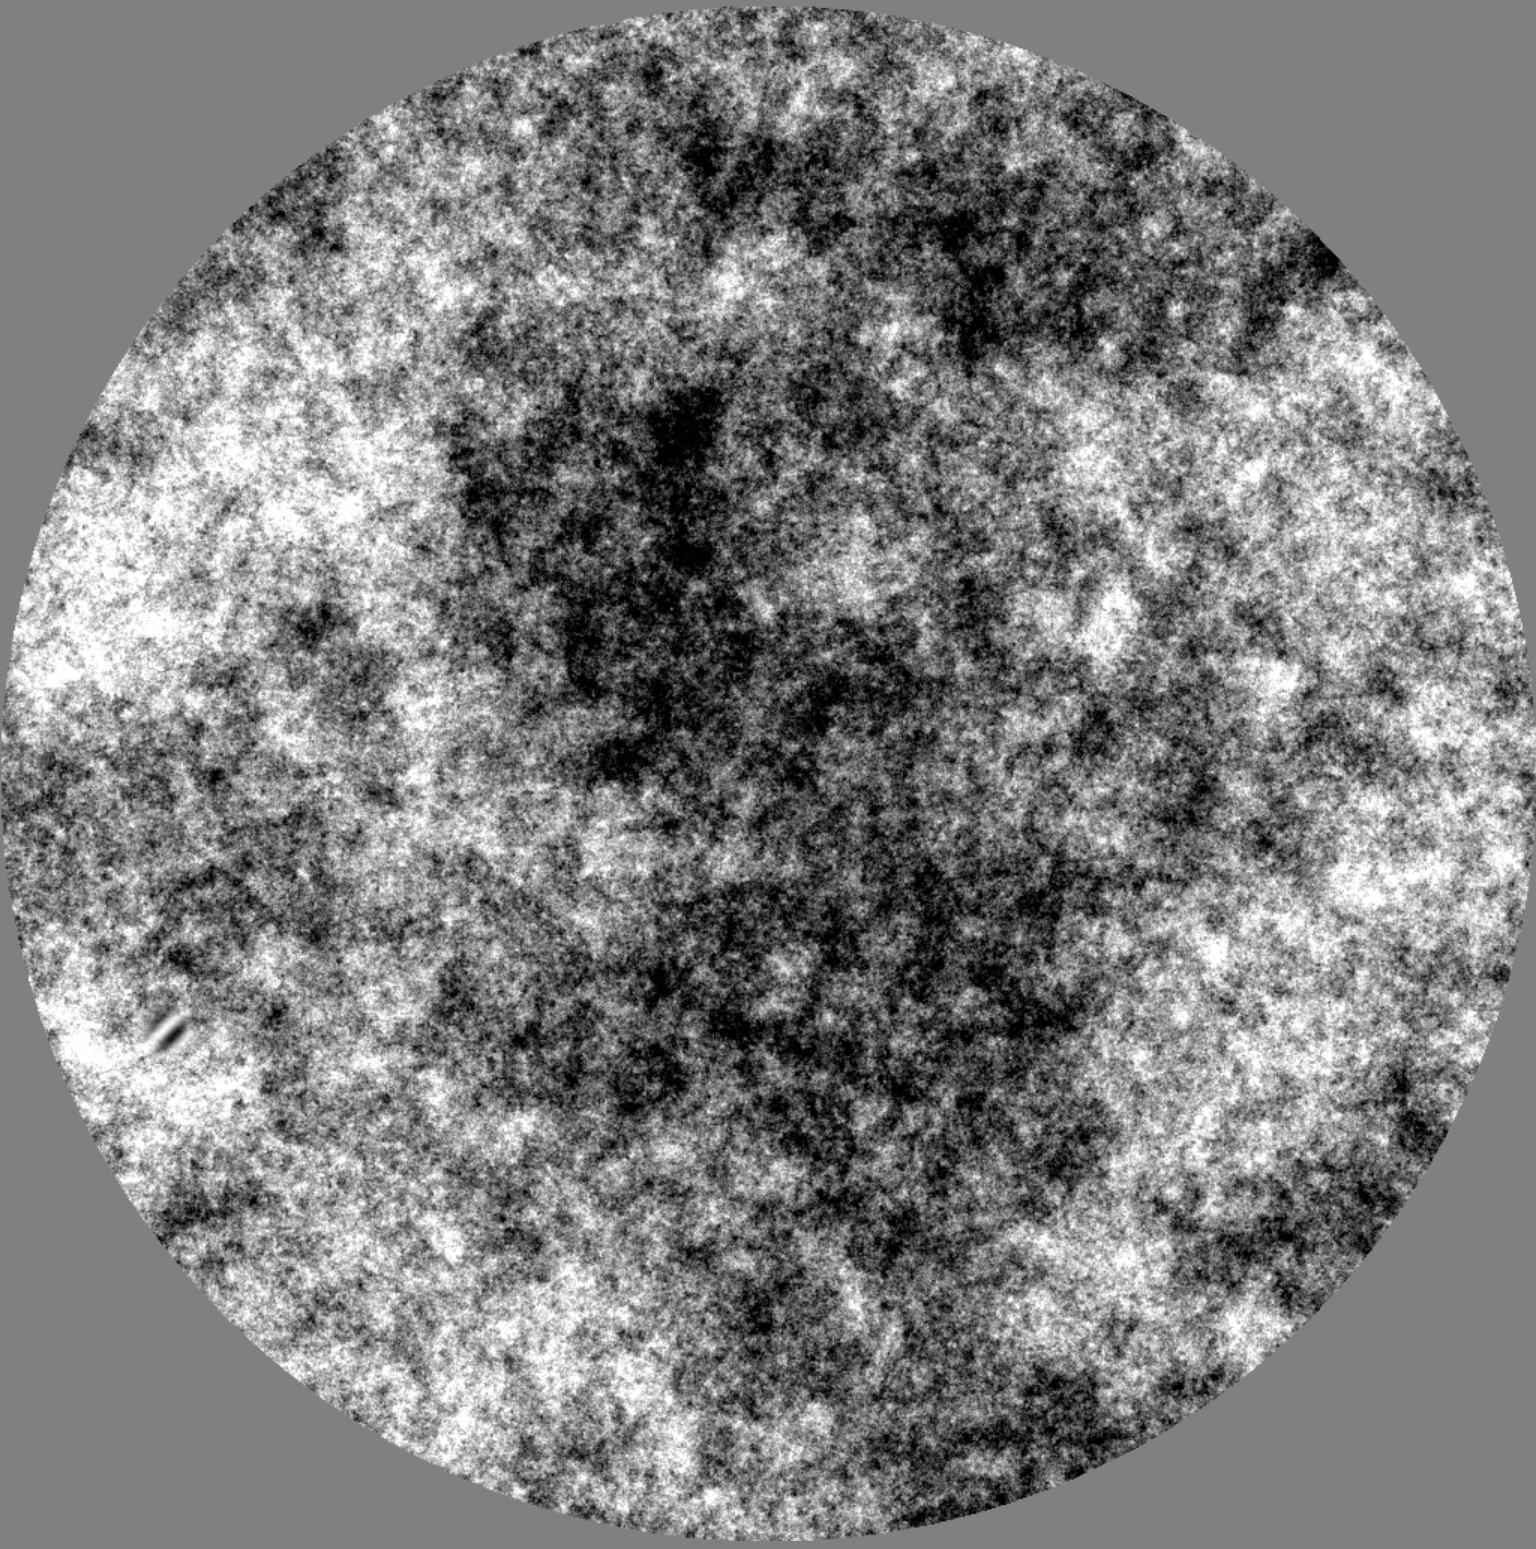
\includegraphics[width = .75\linewidth]{img/noise_visible}
\caption{Šum s dobře viditelným Gabor patchem u levého dolního okraje (kontrast $0.99$).}
\end{subfigure}\\
\noalign{\vskip\bigskipamount}
\\
\begin{subfigure}{0.95\textwidth}
\centering
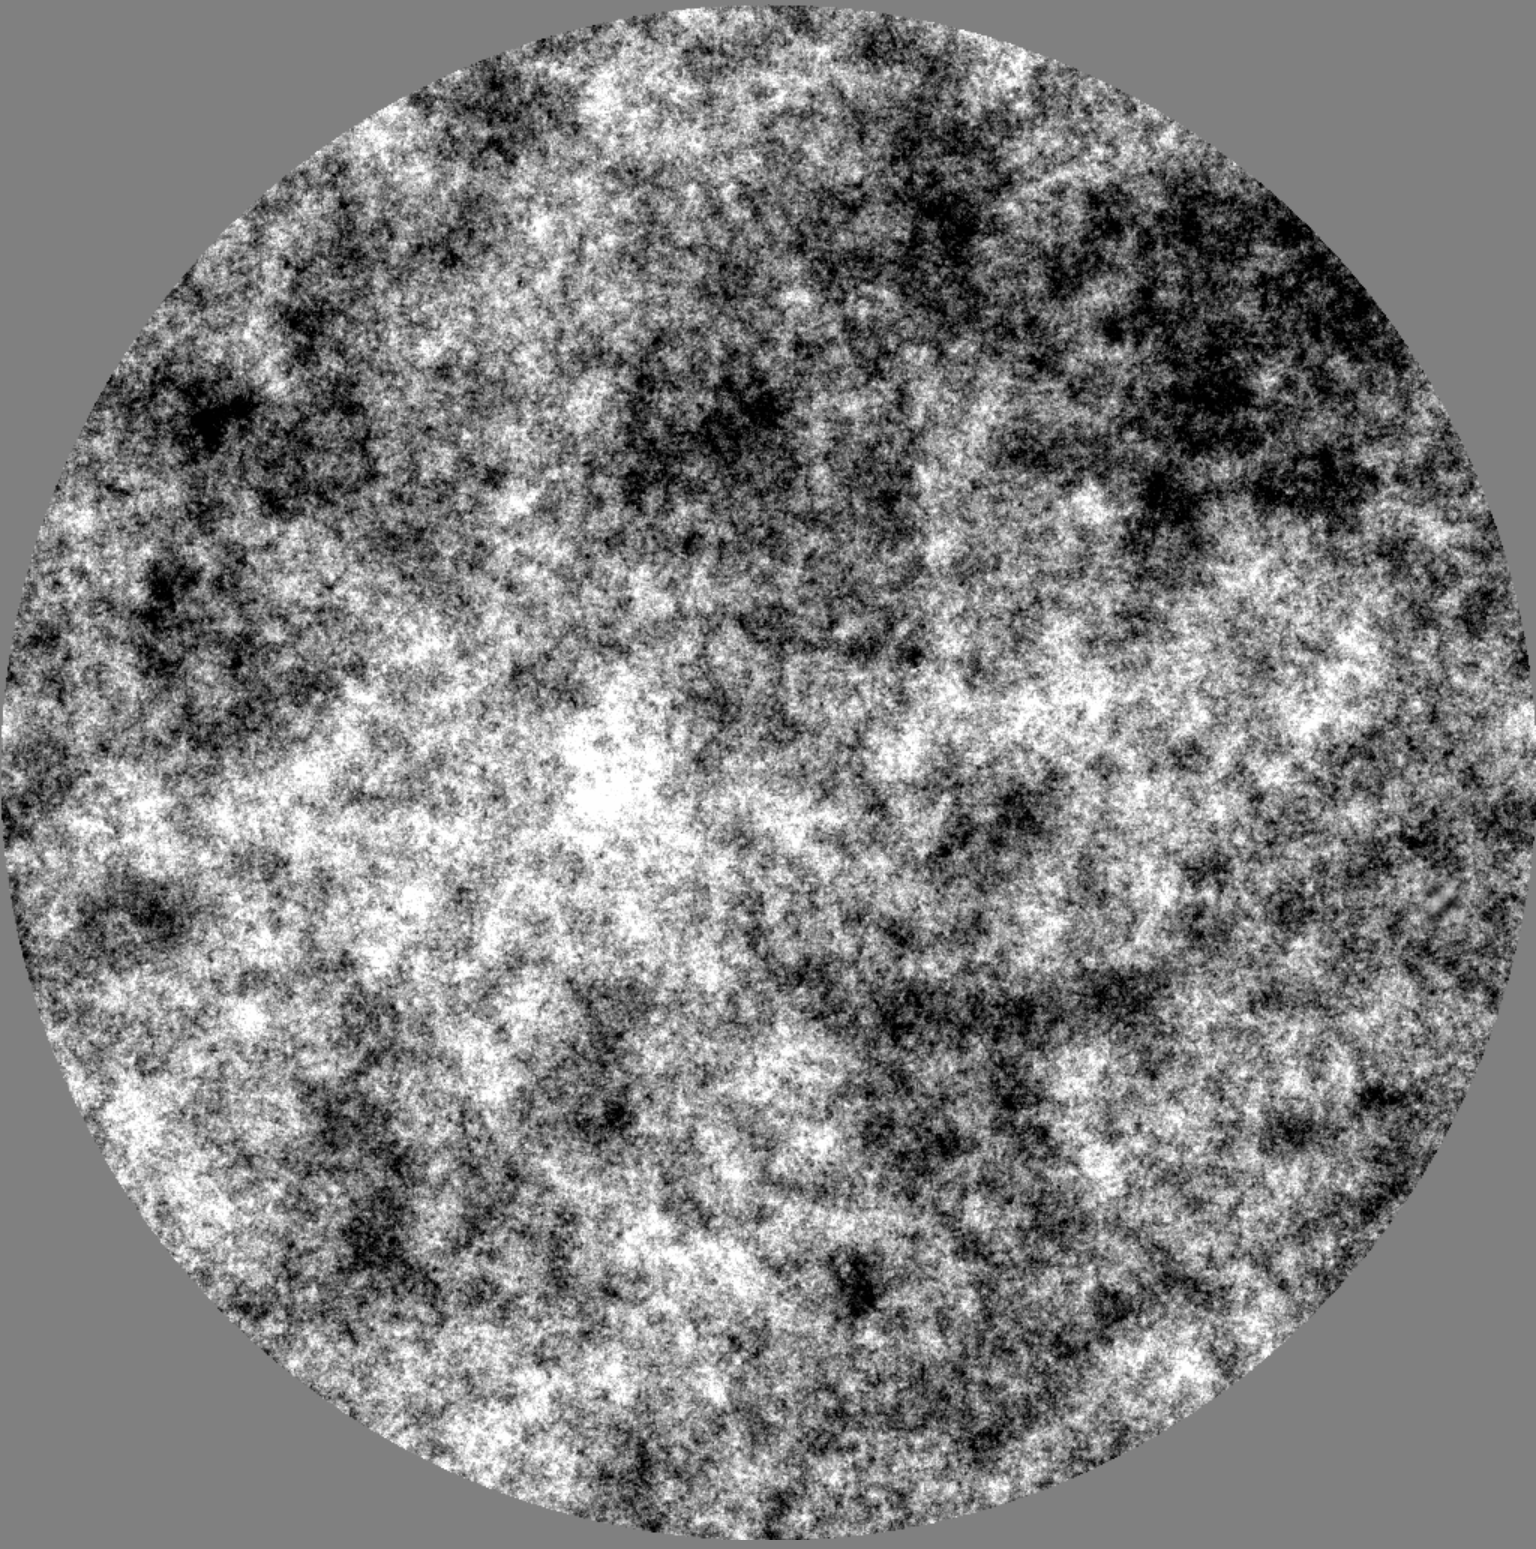
\includegraphics[width = .75\linewidth]{img/noise_invisible}
\caption{Šum se špatně viditelným Gabor patchem u pravého okraje (kontrast $0.61$).}
\end{subfigure}
\end{tabular}
\caption{Příklady růžových šumů. Pozice cílů jsou na obou obrázcích zvýrazněny červenou šipkou.}
\label{Sumy}
\end{figure}

K experimentu byla použita aplikace, která je součástí této práce. 
Jako zobrazovací zařízení byl použit iPad air s displejem o rozlišení
$2048\times1536$ a o úhlopříčce $9.7$ palců, což odpovídá rozměrům displeje asi
$19.7 \times 14.8$ centimetrů. Hustota pixelů je 264 pixelů na palec. 

V experimentu použitý růžový šum byl kruhový o průměru 1024 pixelů.\footnote{Odsud již všude, kde není zřejmý opak, se pixelem myslí
pixel obrázku, nikoliv pixel displeje.} Tento průměr byl zvolen proto, že je
to nejbližší mocnina dvojky ke kratšímu rozměr displeje iPadu v pixelech.
Mocnina dvojky byla žádoucí kvůli použití rychlé Fourierovy transformace při
generování růžového šumu. RMS kontrast\footnote{{\it RMS kontrast} je pro
černobílý obraz vlastně jiný název pro standardní odchylku jasu pixelu, kdy jas
měříme tak, aby černý pixel dostal hodnotu nula a bílý hodnotu jedna
\citep{RMS}.} šumu byl po vygenerování roven $0.25$, ale při zobrazování byly
hodnoty lišící se od střední hodnoty o více než dvě standardní odchylky
přiblíženy ke střední hodnotě právě na tuto vzdálenost, čímž byl RMS kontrast
mírně snížen (pro příklad šumu takového, jaký byl použit, viz obrázek \ref{Sumy}). \index{RMS kontrast}

Jako stimulus byl použit Gabor patch. Jedním z problémů aditivního Gabor patche
ale je fakt, že jas pixelu je v praxi omezený. Kdybychom tedy přičítali Gabor
patch k šumu v místě, které má samo o sobě vysoký jas, museli bychom jeho nejvyšší
bod snížit tak, aby součet se šumem nepřesáhl maximální hodnotu jasu pixelu.
Obdobný problém bychom měli s oblastí s nízkým jasem. Tento problém byl vyřešen
tak, že Gabor k šumu nebyl přičten k šumu, ale vložen do něj, jako
kdybychom kreslili Gabor patch přes šum a obálka zastupovala alfa kanál. To
znamená, že jas pixelu v bodě $x$ byl spočítán jako $S[x] \cdot (1-o[x]) +
G[x]\cdot o[x]$, kde $S[x]$ je hodnota šumu v bodě $x$, a $G[x]$ a $o[x]$ jsou
hodnoty Gaboru a jeho obálky.  Zvolené parametry Gabor patche byly:

\begin{itemize}
\item Obálka: Raised cosine
\item Průměr: 50 pixelů
\item Frekvence: $1/16$ cyklu na pixel
\item Fázový posun: 0
\item Úhel $\Theta$: $135^\circ$ 
\end{itemize}

\begin{figure}
\centering
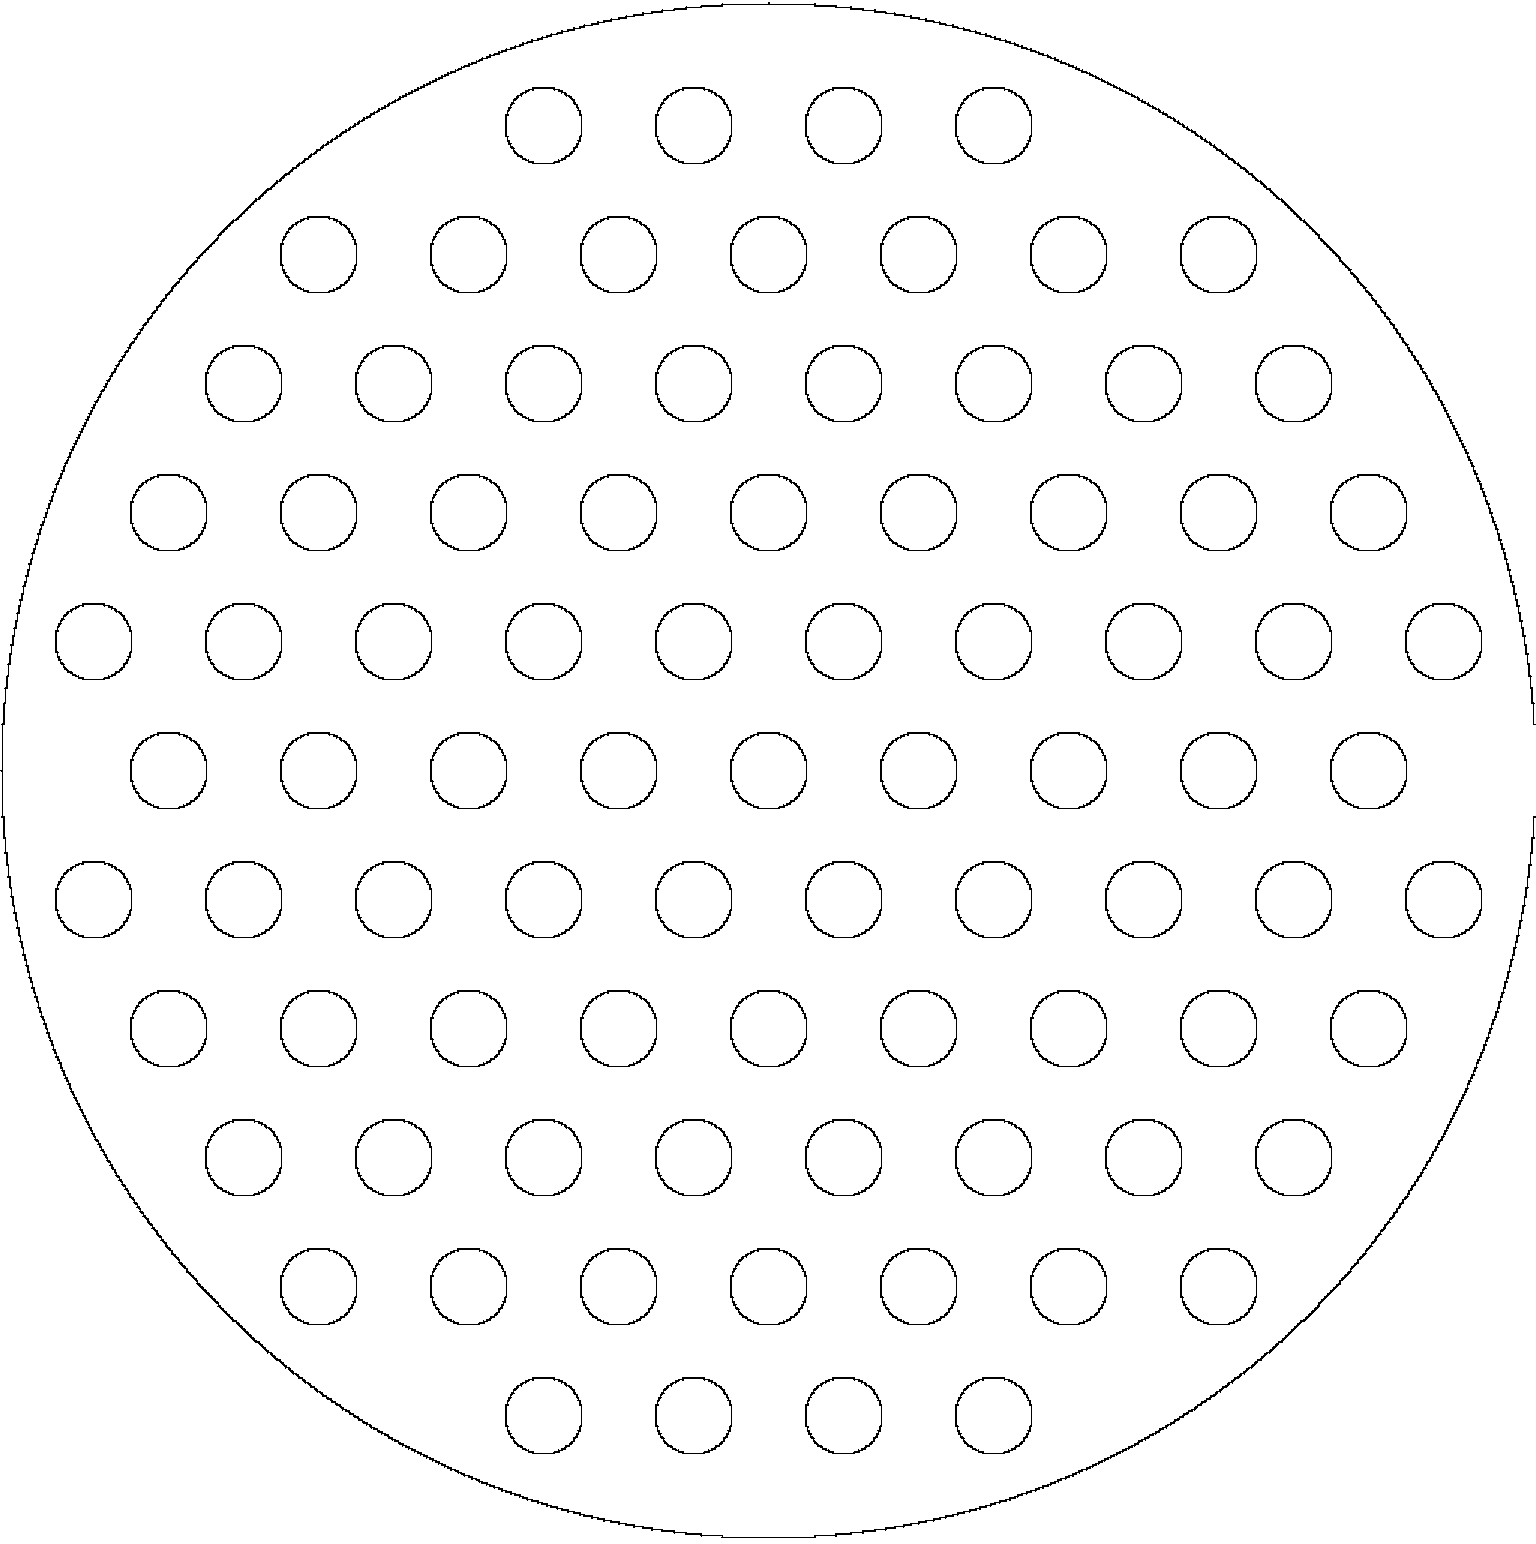
\includegraphics[width=0.48\textwidth]{img/locations_outline.png}
\caption {Možné lokace Gabor patche}.
\label{LokaceGP}
\end{figure}

Možných lokací Gabor patche bylo celkem 85, a byly rozmístěny po scéně v
trojúhelníkové mřížce tak, aby jedna možná lokace byla ve středu. Vzdálenost
dvou sousedních možných lokací byla 100 pixelů (viz obrázek \ref{LokaceGP}). 

Kontrast cíle byl daný maximem obálky, tedy při snižování kontrastu byl cíl čím
dál tím průhlednější. Hodnoty kontrastu se mohly pohybovat mezi nulou a
jedničkou.

Použitá aplikace umožňuje při hledání cíle i počítání skóre, čímž se ze
zrakového vyhledávání stává hra. Tato funkce však byla pro potřeby experimentu
z důvodu úspory času vypnuta. 

\section{Procedura}

Každý účastník prošel sadou 3 testů. V prvním testu mu bylo postupně
prezentováno 40 úkolů, kde v každém z nich měl najít Gabor patch v růžovém
šumu.  V druhém testu bylo prezentováno 120 obdobných úkolů a ve třetím opět
40. 

Ve druhém testu dostávali účastníci, kteří byli ve skupině se zpětnou
vazbou, po každé fixaci zvukovou odpověď, která značila, kolik informace mohli
od této fixace očekávat (tedy jestli bylo z pohledu ELM moudré udělat právě
tuto fixaci). Tato odpověď byla ve formě tónu, jehož frekvence $f$ byla dána
vzorcem $$f = 440\operatorname{Hz}\cdot2^{2-2\cdot\frac{c - \delta}{\Delta -
\delta}},$$ kde $c$ je očekávané snížení entropie při fixaci, kterou si subjekt
vybral, $\Delta$ je maximální dosažitelné očekávané snížení entropie a $\delta$
minimální v případě, že by byla zafixována některá z možných lokací
cíle.\footnote{To znamená, že je potenciálně možné dosáhnout výsledku lepšího
než $\Delta$, resp. horšího, než $\delta$. Rozdíl by však neměl být důležitý.} 

Tento vzorec byl sestaven tak, aby účastník dostal tón a1 v případě, že zvolil
lokaci, která vedla ke stejnému očekávanému snížení entropie, jako lokace
kterou vybral model ELM jako nejlepší, tón a3 v případě, že naopak zvolil
nějakou z nejhorších možných lokací.

V každém úkolu byl šum překryt černou barvou. Subjekt se měl vždy dotknout
displeje v místě, které se rozhodl zafixovat. Na tomto místě byl poté šum
odkryt na $300 \operatorname{ms}$. Výpočet tvaru a míry odkrytí oblasti bylo
provedeno vynásobením s $d'$ mapou posunutou do bodu fixace, s parametrem
$d'_0$ nastaveným na 1 a ostatními parametry naměřenými na pozorovateli FD
($e_R=223$, $e_L=223$, $e_U = 161$, $e_D = 164$, $\beta=2.46$, všechny
veličiny, u nichž má smysl uvádět jednotku, jsou v pixelech; vizualizace viz obrázek \ref{Sumdprime}).

\begin{figure}
\centering
\includegraphics[width = .75\linewidth]{img/noise_d}
\caption{Zakrytý šum s částí odkrytou podle v experimentu použité $d'$ mapy.}
\label{Sumdprime}
\end{figure}

Tuto $d'$ mapu\index{d' mapa@$d'$ mapa} by bylo lepší měřit každému účastníkovi
zvlášť. Stanovení $d'$ mapy ale zahrnuje podle metodiky z článku \citep{Ellipse}
přinejmenším 2000 měření a s metodikou předepsanými přestávkami trvá celý den.
Aby při něm bylo možné kontrolovat chování účastníka, je navíc potřeba
eyetracker. Proto jsme se rozhodli i vzhledem k nemožnosti kontrolovat přesně
podmínky k tomuto měření nepřistoupit. K tomuto problému se ale znovu vrátíme
v diskusi.  

Ve chvíli, kdy si účastník myslel, že objevil cíl, zmáčkl tlačítko. Poté mu byl
ukázán celý odkrytý šum, ovšem bez cíle. Potom se měl účastník dotknout šumu na
místě, kde si myslel, že se cíl nacházel. Cíl byl považován za nalezený, pokud
byla vzdálenost vybraného místa a středu skutečné lokace cíle menší než 60
pixelů displeje, což odpovídá asi $11.5 \operatorname{mm}$. Úkol byl považován za úspěšně splněný, pokud byl cíl nalezen a
současně v rámci něj účastník provedl nejvýše šest fixací. 

V každém testu byl počáteční kontrast cíle $0.7$. Pokaždé, když byl účastník
třikrát po sobě úspěšný, byla zvýšena obtížnost snížením kontrastu cíle o
$0.01$, pokud byl třikrát po sobě neúspěšný, byla obtížnost opět snížena. 

Byl tedy využit obecný postup, kterému se říká Up/Down metoda. Tento postup se
používá, pokud je závislost pravděpodobnosti daného jevu na nějakém parametru
rostoucí (či obecně monotónní) funkce. Spočívá v tom, že se daný parametr
snižuje, když jev nastává, a zvyšuje, když nenastává (v obou případech o předem
danou konstantu, která se během experimentu nemění, nemusí však být v obou
směrech stejná). Blíže je popsána v knize Psychophysics: A practical
introduction \citep{psychophysics}.  Na rozdíl od implementace této metody,
která je popsaná v knize, jsme se rozhodli za jev považovat tři úspěchy za
sebou a za jeho absenci tři neúspěchy, abychom zmenšili velký rozptyl, který
náš jev jinak má.

Hodnota $0.01$ byla vybrána tak, aby se během 120 úkolů, které jsou v
prostředním testu, účastník mohl teoreticky dostat až na hodnoty kontrastu
kolem $0.3$. S kontrastem menším než přibližně $0.45$ je ale pravděpodobnost
splnění úkolu bez ohledu na strategii podle subjektivního názoru autora práce
velmi nízká. V experimentu se tento dojem potvrdil, nejnižší v experimentu
dosažený kontrast byl $0.5$.




\chapter{Měření}

V této kapitole stručně představíme výsledky měření, detailní grafy ke každému pozorovateli zvlášť jsou v první příloze této práce.

\section{Výsledky}
\begin{figure}[h!]
\centering
\begin{tabular}{c}
\begin{subfigure}{0.80\textwidth}
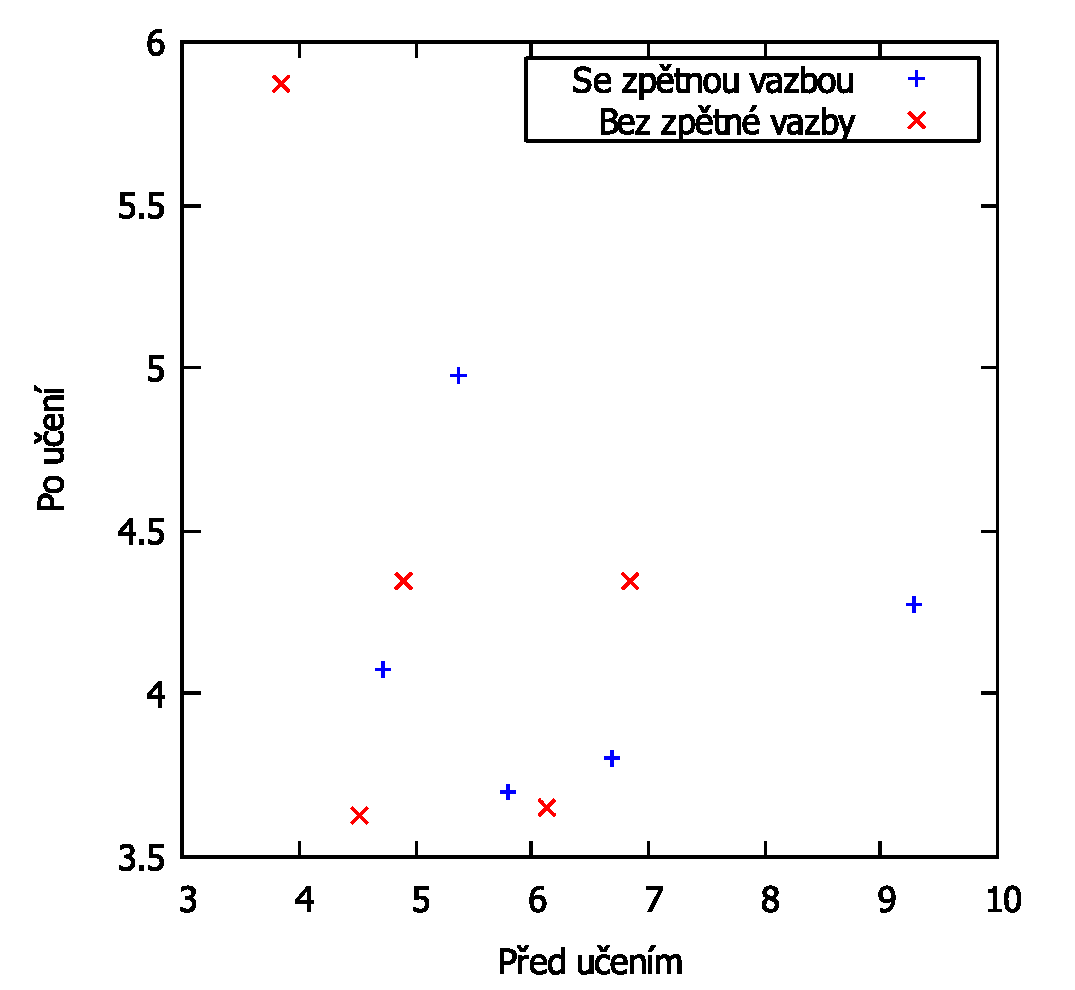
\includegraphics[width=0.99\linewidth]{graphs/AverageTries}
\caption{Průměrný počet fixací}
\end{subfigure}\\
\end{tabular}
\end{figure}
\begin{figure}[h!]
\begin{tabular}{c}
\begin{subfigure}{0.80\textwidth}
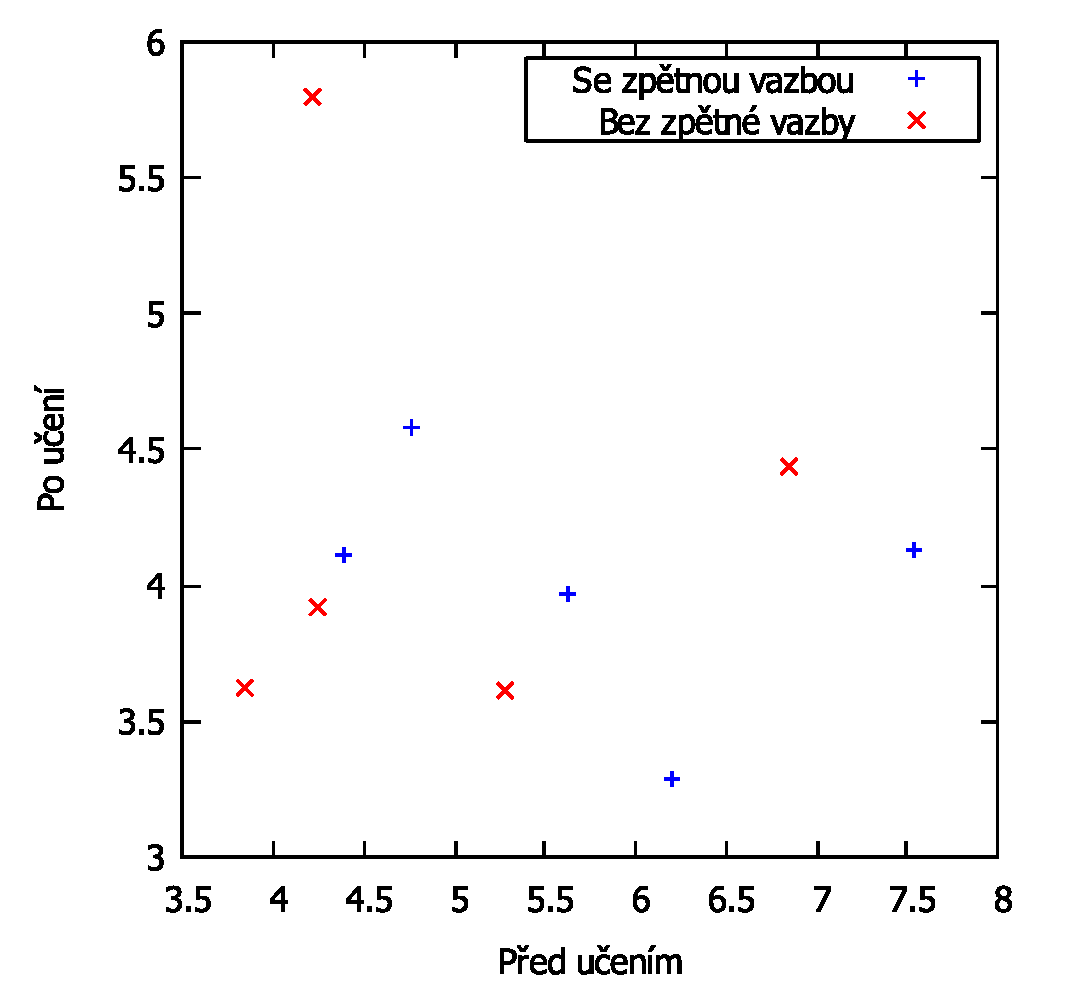
\includegraphics[width=0.99\linewidth]{graphs/AverageSuccesfullTries}
\caption{Průměrný počet fixací v úspěšně splněných úkolech}
\end{subfigure}\\

\begin{subfigure}{0.80\textwidth}
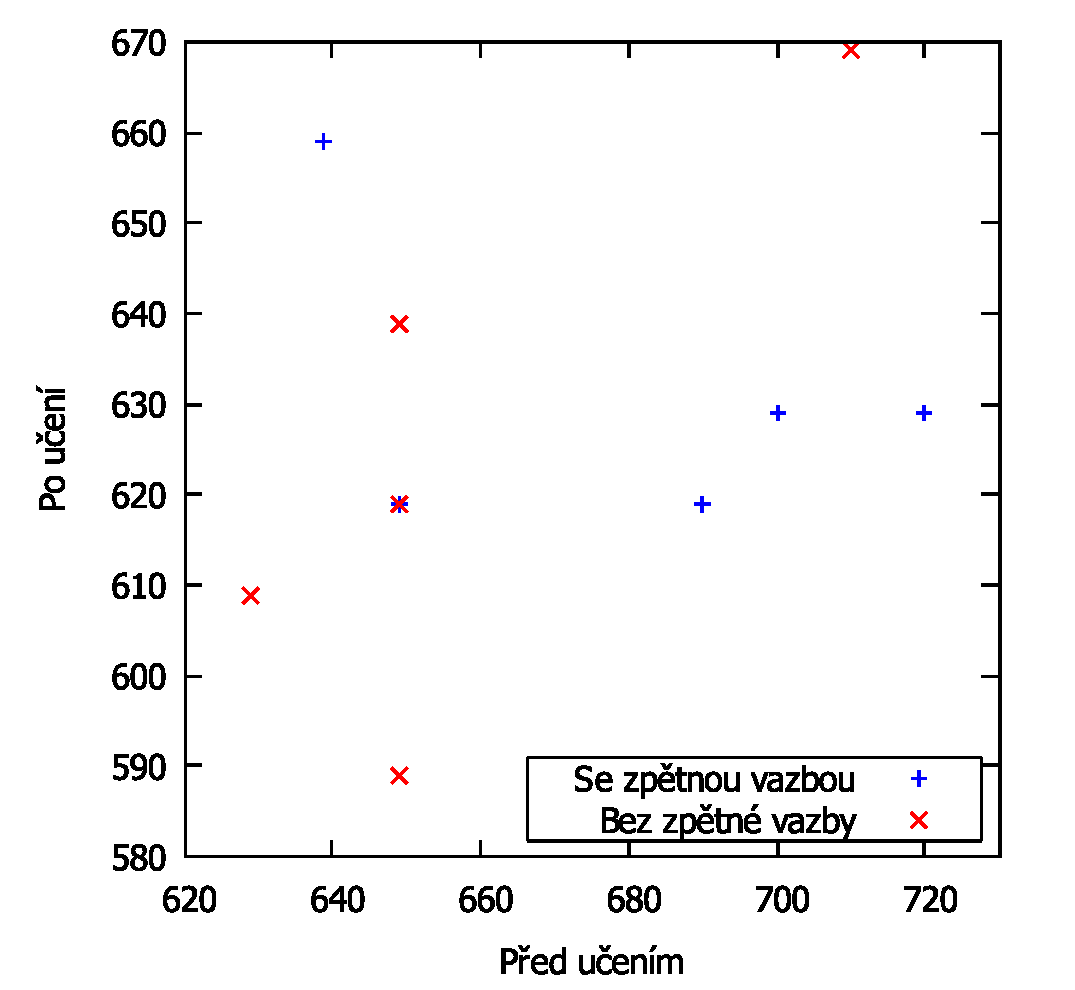
\includegraphics[width=0.99\linewidth]{graphs/FinalDifficulty}
\caption{Obtížnost po 40. pokusu}
\end{subfigure}\\


\end{tabular}
\end{figure}

\chapter{Diskuse}

Cílem experimentu bylo ukázat, zda má zpětná vazba vliv na to, jak dobře se
člověk během daného počtu pokusů naučí hledat cíl.

Analýza naznačuje, že během 120 tréninkových pokusů dochází k měřitelnému a
statisticky významnému zlepšení. Pokud budeme jako jeho ukazatel brát průměrnou
obtížnost, zjistíme, že velikost efektu $\eta^2_p$ dosáhla hodnoty $0.71$,
přičemž velikost daného jevu se hodnotí jako velká od hodnoty $\eta^2_p=0.14$
\citep{Cohen}. Zlepšení je tak výrazné, že i přes relativně malý počet vzorků
vyšla $p$-hodnota $0.002$, což znamená, že hypotézu, že by k učení vůbec
nedocházelo, můžeme zavrhnout nejen na $95\%$ konfidenční hladině, ale i na
$99\%$. Zpětná vazba má na učení nejspíš vliv také. Dosavadní data dokonce
naznačují, že stále velký, a to bez ohledu na to, zda jako ukazatel zlepšení
vezmeme průměrnou obtížnost nebo průměrný počet fixací. Kvůli velkému rozptylu
a malému vzorku se nám však existenci tohoto efektu nepodařilo prokázat
statisticky významně.

Další zajímavou otázkou je, zda byl v experimentu nějak závislý průměrný počet
fixací na kontrastu cíle. Na tuto otázku je na první pohled překvapivá odpověď,
že na sobě tyto dvě veličiny závislé nejsou, nebo jen zcela minimálně --
korelace kontrastu cíle a průměrného počtu fixací je $-0.06$. Další hodnoty
jsou vidět na grafu v první příloze (viz obrázek \ref{kontr}), ale krom
extrémních hodnot kontrastu jsou i na grafu přesně, jak napovídá korelace,
všechny průměry přibližně stejné.

Tento závěr by nás však neměl příliš překvapit, dal se očekávat již při návrhu
experimentu. V experimentu totiž účastníci zústali na dané úrovni kontrastu,
dokud se jim na ní nezačalo výrazněji dařit. Jakmile začali dosahovat dobrých
výsledků, byli přesunuti o úroveň níž. Na místě je otázka, jak bychom tedy měli
navrhnout experiment, jehož cílem by bylo prokázat závěry této práce
statisticky signifikantně. Jedna možnost   

\section{Limitace}

Při návrhu experimentu jsme narazili na několik problémů, které mohly
nepřesnosti do měření, ale jejichž řešení je mimo rozsah této práce. Konkrétně
se jedná o následující obtíže:

\begin{itemize}

\item Vjemy lidského pozorovatele neodpovídají příliš dobře vjemům simulovaného
ideálního pozorovatele. Aby si tyto vjemy odpovídaly, alespoň přibližné, museli
bychom každému pozorovateli změřit jeho vlastní $d'$ mapu. Měření $d'$ mapy ale
i  v té nejminimalističtější variantě, která se používá, trvá nejméně jeden
pracovní den. Druhým důvodem, proč mohou být vjemy rozdílné i v případě, že by
konstanty $d'$ mapy vyšly pozorovateli stejně, jaké byly použity, je, že tato
naměřená $d'$ mapa odpovídá situaci, kdy je scéna se šumem umístěna tak daleko
od pozorovatele, aby ji viděl pod zorným úhlem $15^\circ$. To při velikosti
scény v našem případě odpovídá vzdálenosti pozorovatele a zařízení přibližně
$65 \operatorname{cm}$. V našich experimentech nebyla vzdálenost pozorovatele od
scény hlídána a určitě byla nižší než řečených $65 \operatorname{cm}$
(dodržení této vzdálenosti by odpovídalo situaci, kdy by účastníci drželi iPad
před sebou zhruba na délku natažené paže). 

\item I pokud odhlédneme od nepřesností zmíněných v předchozím bodě a dovolíme
si na chvíli (evidentně scestný) předpoklad, že účastnící měli vlastní $d'$ mapu
konstantní, narazíme na další problém. Okraj oblasti, která byla odkrývána,
byl ztmavován lineárně se snižující se hodnotou $d'$ v použité $d'$ mapě.
Závislost $d'$ na kontrastu ale téměř jistě
není lineární.

\item S tím souvisí ještě jeden problém: Subjekty samozřejmě nemají svou $d'$
mapu konstantní. Tato mapa se tedy nějak skládá s $d'$ mapou, pomocí které
bylo určeno odhalování šumu. V práci jsme toto skládání ignorovali (tedy
předpokládali jsme, že $d'$ na kontrastu závisí lineárně a $d'$ mapa účastníků
je konstantní.) Nabízela by se otázka, proč tedy bylo zatemňování šumu vůbec
prováděno. To se dělo z několika důvodů:

\begin{itemize}

\item Zatemňování šumu zavádí potřebu klikat na místa, která chce pozorovat v
dalším kroku prozkoumat. Nutí tedy pozorovatele, aby tato rozhodnutí dělal
vědomě a nikoli podvědomě, což byl jeden z efektů, které jsme chtěli zkoumat.

\item Celý proces jedné fixace tímto způsobem také trvá mnohem déle (nižší
jednotky vteřin místo nižších desetin vteřiny) a poskytuje nám tedy mnoho času
na update mapy aposteriorních pravděpodobností a výpočet množství informace,
kterou lze získat následující fixací.

\item Takto navržený experiment též umožňuje zjišťovat, které lokace účastník
fixuje bez použití eyetrackeru nebo jiných technologií.

\end{itemize}

\item Zpomalení celého procesu výběru fixace přináší ale i jednu komplikaci. V případě, kdy
účastník provádí jednu fixaci za $300\operatorname{ms}$, nestíhá nad svou
strategií volení fixací přemýšlet. To znamená, že zlepšení strategie je
skutečně způsobeno převážně percepčním učením. V našem experimentu si však
účastníci mohli nad každou další fixací přemýšlet, je tedy pravděpodobné, že
docházelo vedle možného percepčního učení  i ke kognitivnímu učení. Percepční
učení se však v experimentu odehrálo určitě též.  Během experimentu se u
účastníků zjevně podstatně zlepšila jejich senzitivita, ke konci experimentu
byli schopní odhalit cíl s výrazně nižším kontrastem, než na jeho počátku.


\item Vzhledem k tomu, že počet reálných pixelů displeje neodpovídal (a ani
nebyl dělitelný) velikostí scény v pixelech, je možné, že byly efekty jako
například antialiasingem změněny lokální kontrasty scény.

\item Ve výzkumu v oblasti psychofyziky se většinou
pečlivě kontroluje prostředí (například se zatemňuje místnost, v níž se provádí experiment). To jsme v našem výzkumu nedělali.

\end{itemize}

Za zásadní chybu naopak nepovažujeme malý počet účastníků -- kdybychom chtěli
na této práci postavit přesný experiment, nebylo by potřeba zvyšovat počet
účastníků. Jinou, v oblasti psychofyziky často preferovanou cestou, je pokusit
se co nejvíce minimalizovat vliv vnějšího šumu a provádět více měření měření na
jednotlivých účastnících. To bychom mohli uskutečnit například tak, že bychom
vícekrát opakovali první a třetí test. Přístupu, kdy zkoumáme malý počet
účastníků, ale provádíme mnoho co nejpřesnějších měření, se říká small-$N$
design. O jeho výhodách pojednává ve svém článku \citet{SmallN}. Kdybychom se
však rozhodli raději pro Large-$N$ design, mohli bychom většinu ostatních
parametrů experimentu ponechat, ale bylo by potřeba přinejmenším o řád více
účastníků.

V průběhu měření se ukázala jedna chyba v návrhu experimentu, kterou by
bylo při pokračování ve výzkumu vhodné odstranit bez ohledu na to, zda bychom
zvolili small-$N$ či large-$N$ design. 

V aplikaci, pomocí níž byl experiment prováděn, byl naimplementován model obecný
model pozorovatele tak, jak je popsán v článku \citep{Najemnik05}. Tento model
funguje tak, že pozorovatel dostane po fixaci z každé lokace odpověď, která je
číslem náhodně vygenerovaným z normálního rozdělení. Střední hodnota tohoto
rozdělení závisí na tom, zda je v dané lokaci cíl přítomen nebo ne, směrodatná
odchylka závisí na hodnotě $d'$, kterou tato lokace zhledem k zafixované lokaci
má. Takto získané odpovědi potom model použil k update mapy posteriorních
pravděpodobností.

Tento přístup dává smysl v případě, kdy je naším cílem skutečně simulovat
reálného pozorovatele. Reálnému pozorovateli se stejně jako takto simulovanému
občas stane, že vjem z nějaké lokace (typicky dále od místa, které zafixoval,
kde hodnota $d'$ není příliš vysoká) nesprávně vyhodnotí jako pravděpodobnou lokaci
cíle. V takovém případě je samozřejmě racionální následující fixací
zkontrolovat, zda se tam cíl skutečně nachází. Problém nastává ve chvíli, kdy
se takovéhle zavádějící pozorování stane simulovanému pozorovateli, ne však
pozorovateli reálnému. Simulovaný pozorovatel potom svou zpětnou vazbou trvá na
tom, že místo, kde si myslí, že zaznamenal cíl, je nejvhodnější k další fixaci,
často s velkým rozdílem oproti ostatním lokacím. V takové situaci je zpětná
vazba modelu ELM vyloženě matoucí. 

Při opakování experimentu by tedy bylo vhodnější implementovat ELM pozorovatele
tak, aby si myslel, že dostává od modelu odpovědi vybrané z příslušných
distribucí, ve skutečnosti by ale dostával pouze dvě možné konstanty, jednu z
lokací, kde cíl není, a druhou z lokace, kde je. Takto naimplementovaný
pozorovatel by se stále choval dostatečně podobně reálným pozorovatelům, aby
dávalo smysl snažit se naučit lidského pozorovatele jeho strategii, ale zmenšil
by se rozptyl mezi vnitřním šumem pozorovatele a vnitřním šumem modelu.



\chapter*{Závěr}
\addcontentsline{toc}{chapter}{Závěr}

V~práci jsme představili úlohu zrakového vyhledávání, modely několika pozorovatelů
řešících jednu instanci této úlohy a několik dalších souvisejících konceptů a
teorií. Dále jsme popsali principy percepčního učení.

Poté jsme představili hypotézu, která říkala, že se lidé dokážou naučit řešit
úlohu zrakového vyhledávání lépe, pokud budou dostávat po každém pohledu
zpětnou vazbu. Navrhli jsme experiment, ve kterém jsme se snažili tuto hypotézu
potvrdit či vyvrátit. Ten spočíval v~tom, že jsme nechali účastníky experimentu
opakovaně hledat cíl ve scéně s~vizuálním šumem. Nejprve jsme na několika
takových úkolech změřili výkonnost pozorovatele, potom jsme nechali účastníky
na další sadě úkolů trénovat a nakonec jsme opět změřili jejich výkonnost.
Někteří z~nich přitom dostávali ve fázi tréninku při každé fixaci zvukovou
zpětnou vazbu popisující, jak vhodnou lokaci si uživatel k~fixaci vybral.
K~hodnocení byl použit jeden z~modelů pozorovatelů, konkrétně ELM pozorovatel, který efektivně aproximuje Ideálního Bayesovského pozorovatele.

Vytvořili jsme aplikaci pro operační systém iOS, která gamifikuje úlohu zrakového vyhledávání. Poté jsme s její pomocí provedli navržený experiment. I~přesto, že jsme experiment prováděli pouze na deseti
účastnících (a tedy jsme porovnávali dvě pětičlenné skupiny), podařilo se nám
získat statisticky významný výsledek ($p$-hodnota $0.002$), který říká, že při
opakovaném absolvování úlohy zrakového vyhledávání dochází ke zlepšení výkonu.

Pozitivní vliv zpětné vazby, ač pravděpodobně též velký ($\eta^2_p = 0.17$), se nám však již nejspíše kvůli
malému vzorku a velkému množství vnějšího šumu při experimentech
nepodařilo prokázat. Bylo by zajímavé opakovat experiment s~několika drobnými
změnami, které jsme navrhli při zpracování a diskutování naměřených hodnot.
Výsledky jednotlivých skupin jsou však dostatečně rozdílné na to, abychom věřili, že pokračování
výzkumu tímto směrem má smysl.


%%% Seznam použité literatury
%%% Seznam použité literatury (bibliografie)
%%%
%%% Pro vytváření bibliografie používáme bibTeX. Ten zpracovává
%%% citace v textu (např. makro \cite{...}) a vyhledává k nim literaturu
%%% v souboru literatura.bib.
%%%
%%% Příkaz \bibliographystyle určuje, jakým stylem budou citovány odkazy
%%% v textu. V závorce je název zvoleného souboru .bst. Styly plainnat
%%% a unsrt jsou standardní součástí latexových distribucí. Styl czplainnat
%%% je dodáván s touto šablonou a bibTeX ho hledá v aktuálním adresáři.

\bibliographystyle{czplainnat}    %% Autor (rok) s českými spojkami
% \bibliographystyle{plainnat}    %% Autor (rok) s anglickými spojkami
% \bibliographystyle{unsrt}       %% [číslo]

\renewcommand{\bibname}{Seznam použité literatury}

%%% Vytvoření seznamu literatury. Pozor, pokud jste necitovali ani jednu
%%% položku, seznam se automaticky vynechá.

\bibliography{literatura}

%%% Kdybyste chtěli bibliografii vytvářet ručně (bez bibTeXu), lze to udělat
%%% následovně. V takovém případě se řiďte normou ISO 690 a zvyklostmi v oboru.

% \begin{thebibliography}{99}
%
% \bibitem{lamport94}
%   {\sc Lamport,} Leslie.
%   \emph{\LaTeX: A Document Preparation System}.
%   2. vydání.
%   Massachusetts: Addison Wesley, 1994.
%   ISBN 0-201-52983-1.
%
% \end{thebibliography}


\problemy
%%% Obrázky v bakalářské práci
%%% (pokud jich je malé množství, obvykle není třeba seznam uvádět)
\listoffigures

%%% Tabulky v bakalářské práci (opět nemusí být nutné uvádět)
%%% U matematických prací může být lepší přemístit seznam tabulek na začátek práce.
%\listoftables

%%% Použité zkratky v bakalářské práci (opět nemusí být nutné uvádět)
%%% U matematických prací může být lepší přemístit seznam zkratek na začátek práce.
\printindex
%%% Přílohy k bakalářské práci, existují-li. Každá příloha musí být alespoň jednou
%%% odkazována z vlastního textu práce. Přílohy se číslují.
%%%
%%% Do tištěné verze se spíše hodí přílohy, které lze číst a prohlížet (dodatečné
%%% tabulky a grafy, různé textové doplňky, ukázky výstupů z počítačových programů,
%%% apod.). Do elektronické verze se hodí přílohy, které budou spíše používány
%%% v elektronické podobě než čteny (zdrojové kódy programů, datové soubory,
%%% interaktivní grafy apod.). Elektronické přílohy se nahrávají do SISu a lze
%%% je také do práce vložit na CD/DVD. Povolené formáty souborů specifikuje
%%% opatření rektora č. 72/2017.
\appendix
\chapter*{Přílohy}
\addcontentsline{toc}{chapter}{Přílohy}

\sekcicka{První příloha -- Detailnější výsledky měření}

\newpage
\sekcicka{Druhá příloha -- Dokumentace aplikace}

V~této příloze stručně popovídáme o~aplikaci, která je součástí této práce. 

\subsection*{Uživatelská dokumentace}

Při spuštění aplikace se uživatel dostane na úvodní stránku, kde lze nastavit
jméno účastníka, a lze z~ní příslušnými tlačítky pokračovat k~vlastnímu
testování, do nastavení nebo na stránku s~popisem úkolu, který účastníka
experimentu čeká.

Na stránce s~popisem úkolu si uživatel může přečíst, co ho čeká. V~horní části
obrazovky je vždy stručný popis části úkolu, a pod ní je šum, který tuto část
úkolu ilustruje. K~další části přejde kliknutím kamkoli na obrazovku. Délka
ukázky se liší podle toho, zda má aktuální uživatel zapnutou zpětnou vazbu --
v~takovém případě jsou na konec přidány ještě čtyři části popisující zvuk. Po
poslední instrukci je uživatel vrácen na obrazovku, ze které se na stránku
s~popisem úkolu dostal (tj. buď na úvodní stránku, nebo do nastavení).

Na stránce s~nastavením je možné měnit mnoho různých parametrů vyhledávání. Pro
replikaci experimentu tak, jak byl prováděn v~této práci, stačí pouze nastavit
jméno, zpětnou vazbu a v~ostatních parametrech nechat defaultní hodnoty.
Následující tabulka však nabízí popis toho, co přesně které nastavítko ovládá.
U~všech nastavítek, u~nichž se ovládá velikost něčeho,
se hodnota nastavuje v~pixelech šumu.
\bigskip

{
\renewcommand{\arraystretch}{2}
\rowcolors{2}{gray!25}{white}
\begin{longtable}{p{0.25\textwidth}p{0.7\textwidth}}
\hline
\hline
\rowcolor{white}
Popisek & Význam \\
\hline
\endfirsthead
\hline
\hline
\rowcolor{white}
Popisek & Význam \\
\hline
\endhead
\hline
\endfoot
\hline
\hline
\endlastfoot

Difficulty & Průhlednost Gabor patche vynásobená tisícem a zaokrouhlená na
jednotky. Editací tohoto pole se změní jak současná obtížnost, tak obtížnost,
na kterou se hledání vrátí na začátku druhého a třetího testu. Hodnota v~poli
při vstupu do nastavení odpovídá první zmíněné obtížnosti.\\

Gabor patch diameter & Průměr obálky Gabor patche. Perioda se automaticky
nastaví na třetinu této hodnoty. \index{Gabor patch}\\

Radius of uncovered area & V~případě, že je vypnuté použití $d'$ mapy\index{d'
mapa@$d'$ mapa}, odkrývá se šum pomocí masky Raised cosine. Zde je možné
nastavit poloměr masky v~tomto případě.\\ 

Area uncovered for (ms) & Čas v~milisekundách, na který se odkryje šum při
doteku.\\

Area uncovered for brief period only & Určuje, zda se šum odkrývá na trvalo (a
jednotlivé doteky se zobrazují současně), nebo pouze na dobu nastavenou
v~předchozím bodě. Při odkrývání natrvalo se však bez ohledu na nastavení vždy
použije k~odkrývání maska Raised cosine.\\

Sound fully relative & Mění způsob, kterým se počítá výška zvuku. Při vypnutém
nastavítku se používá vzorec uvedený v~kapitole Metody. Při zapnutém se
spočítá, kolik možných lokací cíle má z~pohledu ELM vyšší hodnotu, než vybrané
místo. Tón se pak vybere tak, aby jeho frekvence byla mezi $440$ a $1760$
Hertzy a byla exponenciálně závislá na tomto počtu. \\

Possible location distance & Vzdálenost možných lokací cíle \\

Regenerate noise & Návrat k~měření se zapnutou touto možností způsobí kompletní
restart současného úkolu, včetně přegenerování šumu a lokace Gabor patche.
Vhodné zapnout, pokud jsme měnili některá jiná nastavení. \\

Preview & Přesune uživatele na stránku s~popisem úkolu. \\ 

Start game & Zobrazí obrazovku s~experimentem. \\

Back to main menu & Návrat na úvodní obrazovku. \\

Trials in first and third test & Počet úkolů  v~prvním a třetím testu. \\

Trials in second test & Počet úkolů během tréninku. \\

Correct/wrong responses in row before difficulty changes & Počet správných či
špatných odpovědí v~řadě, po kterých se změní obtížnost. \\

Difficulty changed by & O~kolik se změní obtížnost (tisícem vynásobená
průhlednost Gabor patche), když se má měnit (viz předchozí řádek). \\

Accuracy threshold & Maximální chyba v~pixelech displeje, o~kterou se uživatel
může splést, aby byl úkol ještě uznán jako úspěšně splněný. \\

Maximal amount of fixations for succesfull trial & Maximální počet fixací, po
nichž musí být oznámeno nalezení cíle, aby byl úkol považován za úspěšně
splněný. \\

Calculate score? & Vynuluje a zapne počítání a zobrazování skóre. Skóre získané
jedním úkolem je 0, pokud cíl nebyl nalezen, jinak je určeno podle vzorce
$\lfloor(1000 - \text{(Obtížnost)})/\text{(Počet fixací)}\rfloor$. \\

$d'$ map constants settings & Prvních šest nastavení v~této kategorii určuje
přímočarým způsobem konstanty $d'$ mapy tak, jak jsou popsány v~kapitole, která
se jí věnuje. Hodnoty $d'_0$ a $\beta$ je nutné zadávat vynásobené stem. \\

Recalculate $d'$ map & Po změně parametrů $d'$ mapy přepočítá pomocné datové
struktury. Bez stlačení tohoto tlačítka by nemělo být možné po editaci konstant
opustit nastavení. Přepočítávání se neděje automaticky po změně libovolné
hodnoty, protože může trvat až několik vteřin a často je potřeba změnit více
konstant současně. \\

Use $d'$ map & Rozhoduje o~tom, zda bude pro odkrývání šumu použita maska
spočítaná z~$d'$ mapy, nebo Raised cosine.\\

Name & Identifikátor účastníka.\\

Feedback & Zapíná a vypíná zpětnou vazbu pro účastníka v~druhém testu.
V~případě, že je jméno účastníka \uv{unknown}, což je defaultní hodnota, je při
zapnutí této funkce z~ladících a předváděcích důvodů zpětná vazba poskytována
bez ohledu to, v~kterém testu se nachází.\\

Measure detectability & Spustí obrazovku, kde je uživateli prezentována řada
pokusů, kdy se vždy Gabor patch se současnými parametry objeví ve středu
s~pravděpodobností $1/2$. Uživatel pak může otestovat, jakou má při daných
vlastnostech cíle hit rate a false alarm rate.\\

See log & Zobrazí log všech testů od posledního vymazání všech dat. Log zůstává
napříč spuštěními aplikace a ukládá se automaticky po každém dokončeném
úkolu.\\

Data deletion enabled & Je-li tato možnost aktivována, stlačení tlačítka
\uv{Delete all data} opravdu smaže všechna data. V~opačném případě je uživatel
upozorněn na to, že musí mazání dat nejprve povolit.\\

Delete all data & Viz předchozí řádek.\\

Generate noise & V~případě, že je tato funkce vypnutá, bude místo růžového šumu
vygenerována pouze šedá plocha.\\

Display locations & Je-li tato možnost zapnuta, bude v~místě každé lokace
zobrazen světlý kruh. Přesný odstín jeho pravé horní poloviny je závislý na
aposteriorní pravděpodobnosti, kterou ELM pozorovatel přiřazuje právě této
lokaci (čím světlejší půlkruh, tím vyšší pravděpodobnost). Odstín levé dolní
poloviny je závislý na očekávaném snížení entropie, které podle ELM
pozorovatele nastane, zafixujeme-li v~dalším kroku tuto lokaci (opět světlejší
kruh znamená větší očekávané snížení entropie). Ve středu kruhu, kde je
očekávané snížení entropie největší (ve všech takových, není-li to jednoznačné)
se nachází černá tečka. \\

\end{longtable}
 }

\bigskip
V~obrazovce, kde se provádí experiment, se vše koná tak, aby jediný nutný zásah
do experimentu od administrátora byl, že bude sledovat počet uskutečněných
úkolů (napsaný spolu s~dalšími důležitými hodnotami v~horní části obrazovky) a
upozorní účastníka, když má experiment končit. Aplikace sama postupně mění
obtížnost, dává zvukovou zpětnou vazbu v~situacích, kdy má, a restartuje
obtížnost na defaultní hodnotu na začátku druhého a třetího úkolu.

\subsection*{Programátorská dokumentace}

Aplikace je napsána v~jazyce Swift, který je určený pro psaní nativně běžících
aplikací pro operační systém iOS. Je určená na zařízení iPad Air.

V~této sekci stručně přiblížíme dva netriviální algoritmy, které se v~aplikaci
vyskytují Bude se jednat o~výpočet očekávaného snížení entropie v~rámci
simulace ELM pozorovatele, a generování růžového šumu.

V~obou těchto algoritmech je potřeba generovat náhodná čísla s~normálním
rozdělením. Na to použijeme funkci {\tt GKGaussianDistribution.nextUniform()},
která je součástí knihovny {\tt GameplayKit}, jedné ze standardních knihoven
jazyka Swift. Tato funkce se od normálního rozdělení odklání v~tom, že
nepřipouští hodnoty, které se od střední hodnoty rozdělení liší o~více než tři
standardní odchylky. Protože je však pravděpodobnost takových hodnot
v~normálním rozdělení rovna přibližně $0.003$, rozhodli jsme se, že ovlivnění
experimentu touto odlišností zanedbáme.

\subsubsection*{Model ELM pozorovatele}

ELM \index{ELM pozorovatel} byl v~práci vytvořen přesně tak, jak byla jeho simulace popsána v~článku \citep{Najemnik09}. 

To znamená, že při fixaci bodu $x$  dostane z~každé lokace $y$ jako pozorování reálné
číslo, které je náhodně vybrané z~normálního rozdělení, jehož střední hodnota
je $-0.5$, pokud se cíl v~daném bodě nenachází, a $0.5$ pokud ano. Směrodatná
odchylka tohoto rozdělení je rovna hodnotě $d'(y-x)$\index{d'@$d'$}. Poté
spočítá veškerou informaci, kterou již o~jednotlivých lokacích dostal, jako
součet odpovědí, které dostal při předchozích fixacích, vynásobený druhými
mocninami příslušných hodnot $d'$ (ve skutečnosti stačí přičíst odpovědi
z~aktuální fixace k~již spočítanému součtu po předchozí fixaci).

V~dalším kroku spočítá aposteriorní pravděpodobnosti prostě tak že pro získaný
součet $s$ nastaví aposteriorní pravděpodobnost na $e^s$, a pak ještě všechny
aposteriorní pravděpodobnosti vydělí jejich součtem, aby byl po vydělení součet
roven jedné. Až po sem je algoritmus lineární v~počtu možných lokací. Nyní je
však potřeba spočítat očekávané snížení entropie. To se spočítá podle již dříve
uvedeného vzorce jako $$\displaystyle\sum_{i\in L} p_T(i)d'^2(i-k(T+1)),$$ kde
$L$ je množina možných lokací, $p_T(i)$ je aposteriorní pravděpodobnost, že se
cíl nachází v~lokaci $i$ a $k(T+1)$ je lokace, jejíž očekávané snížení entropie
počítáme.   

Před první fixací se očekávaná snížení entropie počítají obdobně, až na to, že
jako pole s~předchozími odpovědi použijeme pole vyplněné samými nulami.

Důkaz korektnosti algoritmu zde nebudeme uvádět, neboť je již uvedený v~článcích \citep{Najemnik05, Najemnik08, Najemnik09}.

\subsubsection*{Generování růžového šumu}

\index{Šum!růžový} 

Šum generujeme tak, že nejprve vygenerujeme dvojrozměrné pole náhodných
komplexních čísel stejně velké, jak velký chceme výsledný šum. Tato komplexní
čísla mají v~goniometrické podobě rovnoměrně náhodné argumenty. Absolutní
hodnotu čísla na pozici $(x,y)$ v~poli $n\times n$ vybereme z~normálního
rozdělení se střední hodnotou \begin{equation}\label{Pink}\left(\min\left(x,n-x\right)^2
+\min\left(x,n-x\right)^2\right)^{-2}\end{equation} a směrodatnou odchylkou rovnou třetině
této hodnoty. V~případě, kdy by tato hodnota vyšla jako nekonečno, můžeme
hodnotu prostě zahodit (zdůvodnění tohoto tvrzení dále vyplyne z~algoritmu) a
použít libovolnou. Výběr střední hodnoty vychází z~definice růžového šumu,
odchylka byla zvolena při testování kvůli výše uvedeným vlastnostem náhodného
generátoru (nemůže se nám stát, že by vyšla záporná absolutní hodnota), a byla
na této hodnotě ponechána, protože algoritmus dával vizuálně žádoucí výsledky a
definice růžového šumu ji nespecifikuje.

Na takto vytvořené pole zavoláme (zpětnou, ale ve skutečnosti na tom nezáleží)
dvojrozměrnou rychlou Fourierovu transformaci\footnote{Dvojrozměrná diskrétní
Fourierova transformace je Fourierova transformace nejprve provedená po řádcích
a potom po sloupcích.}.  Výsledkem je růžový šum. My ho ale potřebujeme být
schopni zobrazit. Nejprve tedy zahodíme imaginární složku komplexních čísel.
Poté spočítáme jeho průměr a směrodatnou odchylku a uplatníme na něj lineární
transformaci takovou, aby jeho střední hodnota byla 128 a směrodatná odchylka
64. Nakonec záporné hodnoty nastavíme na nulu a hodnoty převyšující 255 na 255.
Nakonec nastavíme na 128 ty pixely, jejichž (eukleidovská) vzdálenost od středu
obrazu je větší, než $n/2$, čímž dosáhneme toho, že výsledné pole bude kruhové.
Výsledné pole interpretujeme jako černobílý obraz s~osmi bity na pixel.


Fourierovu transformaci nalezneme v~knihovně {\tt Accelerate}, která je jednou ze
standardních knihoven jazyka Swift.

Nyní se vrátíme k~tomu, proč jsme mohli zahodit hodnotu, pro níž vyšel
nekonečný koeficient. Ten vyjde právě tehdy, když jsou ve vzorci \eqref{Pink}
obě sčítané závorky nulové. Budeme-li $x$ i $y$ indexovat od nuly, znamená to,
že musí být $x$ i $y$ rovno nule. To znamená, že se tato situace týká jednoho
jediného bodu, a to bodu $(0,0)$. Protože ale poté voláme Fourierovu
transformaci, z~nultého bodu se stane hodnota, která se násobí pouze jedničkou,
tedy ji beze změny přičteme ke každé hodnotě. Protože ale potom stejně šum
lineárně transformujeme, aby měl správnou střední hodnotu a směrodatnou
odchylku, žádná předchozí nekonstantní lineární transformace výstup neovlivní
(nebo alespoň ne více, než tím, že způsobí nějaké nechtěné
zaokrouhlování\footnote{V algoritmu je komplexní číslo reprezentováno pomocí
dvou hodnot typu {\tt Double}.}, to ale nebude mít v~praxi významný vliv).

Pro generování jiného z~šumů, o~kterých se mluví v~sekci o~barvách šumu, stačí 
ve vzorci \eqref{Pink} vynásobit hodnotu $-2$ v~exponentu příslušnou hodnotou $\beta$.


\openright
\end{document}
